\chapter{La régulation}

Ce chapitre revient principalement se concentrer sur les travaux réalisés par Laucella \cite{Laucella} et Yersin \cite{Yersin}.

\section{Introduction}
La réalisation du système nécessite une régulation de courant imbriquée dans une régulation de position. Le schéma suivant illustre cette architecture :

\begin{figure}[H]
    \centering
    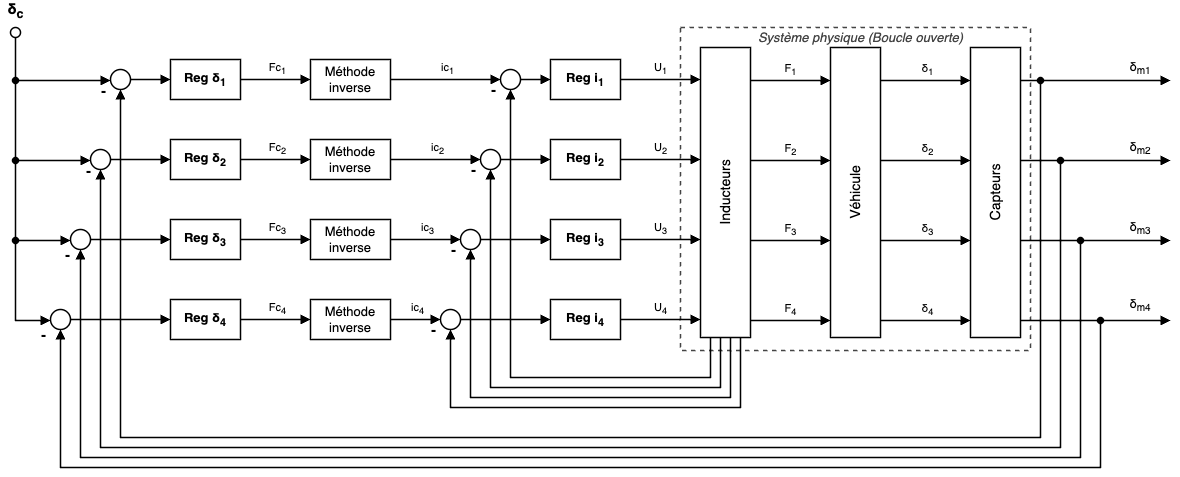
\includegraphics[width=1\linewidth]{assets/Chap4/SchemaBlocRegulationSISO.png}
    \caption{Schéma bloc de la régulation de courant imbriquée position \cite{Laucella}}
    \label{fig:SchemaBlocRégulation}
\end{figure}

Cette disposition permet d'assurer la lévitation de la maquette. La régulation de courant assure le contrôle du courant traversant l'inducteur, tandis que la régulation de position détermine l'élévation de la maquette par la mesure de la distance de l'entrefer.

Les blocs « Reg i1 » à « Reg i4 » représentent la régulation de courant. Une consigne de courant est fournie en entrée et une tension est appliquée aux inducteurs en sortie. Cette régulation de courant est réalisée par un régulateur PI.

Les blocs « Reg $\delta$1 » à « Reg $\delta$4 » représentent la régulation de position. Celle-ci reçoit une position en entrée et génère une force en sortie. Ce contrôle est assuré par une régulation par retour d'état (espace d'état).

Les blocs « méthode inverse » ont pour but de calculer le courant à partir de la force souhaitée par un électroaimant. L'équation mathématique est développée dans la sous-section \ref{subsec:Fele}.

\section{Définition du système}

\subsection{Le système}
Afin de réaliser une synthèse rigoureuse de la régulation, l'élaboration d'un modèle mathématique de la maquette est nécessaire. Le système est ainsi modélisé à travers plusieurs étapes successives permettant d'aboutir aux équations de comportement. Cette démarche permet d'obtenir une formulation globale définissant l'ensemble du système, sur laquelle s'appuiera la synthèse de la régulation.\\

Le système conserve la même définition que lors des travaux précédents, comme illustré par la figure \ref{fig:BobineRep} :

\begin{figure}[H]
    \centering
    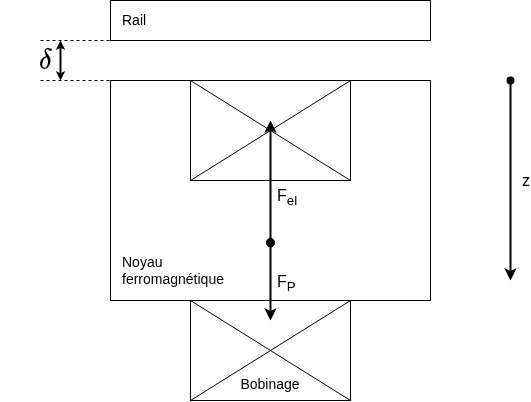
\includegraphics[width=0.75\linewidth]{assets/Chap4/Bobine.png}
    \caption{Représentation de la bobine}
    \label{fig:BobineRep}
\end{figure}

Pour rappel, les différentes grandeurs présentes sur la maquette sont synthétisées dans les tableaux suivants :

\begin{table}[H]
    \centering
    \renewcommand{\arraystretch}{1.2}
    \begin{tabular}{|c|l|c|c|}
        \hline
        \multicolumn{4}{|c|}{\textbf{Paramètres Mécaniques}}                                                  \\ \hline
        \textbf{Symbole} & \textbf{Description de la grandeur}             & \textbf{Valeur} & \textbf{Unité} \\ \hline
        $m_{tot}$        & Masse totale du chariot (actuelle)              & 18.052          & kg             \\ \hline
        $m$              & Masse supportée par 1 inducteur ($m_{tot} / 4$) & 4.513           & kg             \\ \hline
        $g$              & Accélération gravitationnelle                   & 9.81            & m/s$^2$        \\ \hline
    \end{tabular}
    \caption{Paramètres mécaniques de la maquette de sustentation.}
    \label{tab:param_mecaniques}
\end{table}

\begin{table}[H]
    \centering
    \renewcommand{\arraystretch}{1.2}
    \begin{tabular}{|c|l|c|c|}
        \hline
        \multicolumn{4}{|c|}{\textbf{Paramètres de l'Inducteur et de l'Entrefer}}                                                           \\ \hline
        \textbf{Symbole}             & \textbf{Description de la grandeur}                          & \textbf{Valeur}      & \textbf{Unité} \\ \hline
        $N$                          & Nombre de spires de la bobine                                & 125                  & -              \\ \hline
        $R$                          & Résistance de la bobine                                      & 0.8                  & $\Omega$       \\ \hline
        $A$                          & Surface de l'entrefer ($20 \text{ mm} \times 50 \text{ mm}$) & $1 \cdot 10^{-3}$    & m$^2$          \\ \hline
        $\mu_0$                      & Perméabilité du vide                                         & $4\pi \cdot 10^{-7}$ & H/m            \\ \hline
        $\delta_n$                   & Entrefer nominal (consigne)                                  & 2                    & mm             \\ \hline
        $\delta_{max}$ ou $\delta_0$ & Entrefer maximum (chariot posé)                              & 3                    & mm             \\ \hline
        $\delta_{min}$               & Entrefer minimum (structure collée)                          & 0.1                  & mm             \\ \hline
        $U_{d}$                      & Tension d'alimentation du bus DC (PWM)                       & 48                   & V              \\ \hline
    \end{tabular}
    \caption{Paramètres électriques de l'inducteur et caractéristiques de l'entrefer.}
    \label{tab:param_inducteur_entrefer}
\end{table}

\begin{table}[H]
    \centering
    \renewcommand{\arraystretch}{1.2}
    \begin{tabular}{|c|l|c|c|}
        \hline
        \multicolumn{4}{|c|}{\textbf{Paramètres Numériques et Fréquences}}                                      \\ \hline
        \textbf{Symbole} & \textbf{Description de la grandeur}               & \textbf{Valeur} & \textbf{Unité} \\ \hline
        $f_e$            & Fréquence d'échantillonnage et de la PWM          & 25              & kHz            \\ \hline
        $h$              & Période d'échantillonnage ($1 / f_e$)             & 40              & $\mu$s         \\ \hline
        $f_{md}$         & Bande passante du capteur de position (Baumer)    & 1.1             & kHz            \\ \hline
        $f_{mi}$         & Fréquence de coupure retenue pour capteur courant & 25              & kHz            \\ \hline
    \end{tabular}
    \caption{Paramètres d'échantillonnage, traitement numérique et fréquences de coupure.}
    \label{tab:param_numeriques_frequences}
\end{table}

\subsection{Modélisation d'une inductance}
Le contrôle du système reposant sur des bobines, il est nécessaire de définir la valeur de leur inductance. Pour ce faire, les paramètres du tableau \ref{tab:param_inducteur_entrefer} sont employés afin d'effectuer ce calcul.\\

Afin d'alléger les développements, les hypothèses simplificatrices suivantes ont été formulées :
\begin{itemize}
    \item Perméance du fer infinie.
    \item Absence de saturation du fer.
    \item Effets de bord (franges) négligés.
    \item Effet d’hystérésis négligé.
    \item Flux de fuite négligés.
\end{itemize}

Pour commencer, un schéma magnétique a été établi afin d'obtenir une représentation rigoureuse de la perméance du système. Ce tracé respecte les hypothèses énoncées ci-dessus :

\begin{figure}[H]
    \centering
    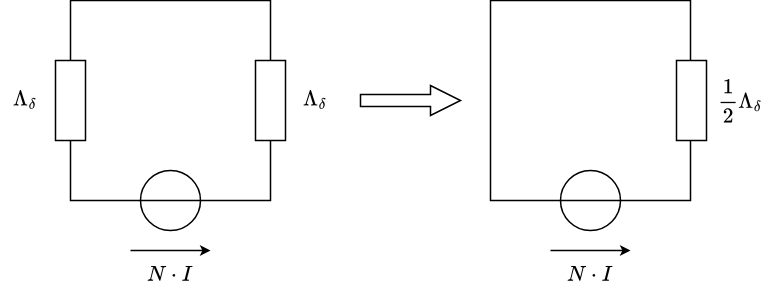
\includegraphics[width=0.8\linewidth]{assets/Chap4/SchemaMagnetique.png}
    \caption{Schéma magnétique}
    \label{fig:SchemaMagnetique}
\end{figure}

À partir de la figure \ref{fig:SchemaMagnetique}, la perméance totale vue par l'enroulement peut être formulée selon l'équation \ref{eq:PermTot} :

\begin{equation}
    \Lambda_{tot} =\frac{1}{2}\cdot \Lambda_{\delta} = \frac{1}{2}\cdot\frac{\mu_0 \cdot A}{\delta} = \frac{\mu_0 \cdot A}{2\cdot\delta}
    \label{eq:PermTot}
\end{equation}

L'inductance se calcule ensuite en injectant l'équation \ref{eq:PermTot} dans la relation \ref{eq:IndAnal} :

\begin{equation}
    L(\delta) = N^2 \cdot \Lambda_{tot} = \frac{1}{2} \cdot N^2 \cdot \Lambda_{\delta} = \frac{N^2 \cdot \mu_0 \cdot A}{2 \cdot \delta}
    \label{eq:IndAnal}
\end{equation}

Le système est défini autour d'un point de fonctionnement nominal, correspondant à l'état stable pour une hauteur de lévitation de 1~mm. Dans cette condition, l'entrefer équivaut à l'entrefer nominal, soit $\delta = \delta_n = 2\text{ mm}$. En repartant de l'équation précédente \ref{eq:IndAnal}, l'inductance nominale s'écrit alors :

\begin{equation}
    L(\delta_n) = L_n = \frac{N^2 \cdot \mu_0 \cdot A}{2 \cdot \delta_n} = \frac{125^2 \cdot 4\pi \cdot 10^{-7} \cdot 10^{-3}}{2 \cdot 2 \cdot 10^{-3}} = 4,9 \text{ mH}
    \label{eq:IndNom}
\end{equation}

De cette équation \ref{eq:IndNom}, il est possible d'isoler la partie constante, qui pourra être employée par la suite pour simplifier l'équation \ref{eq:IndAnal} :

\begin{equation}
    L(\delta_n) = L_n = \frac{N^2 \cdot \mu_0 \cdot A}{2 \cdot \delta_n} \rightarrow L_n \cdot\delta_n = \frac{N^2 \cdot \mu_0 \cdot A}{2}
    \label{eq:Cst}
\end{equation}

Cette relation \ref{eq:Cst} peut être réintroduite dans l'équation \ref{eq:IndAnal}, ce qui donne :

$$L(\delta) = \frac{N^2\cdot \mu_0\cdot A}{2}\cdot \frac{1}{\delta}$$

\begin{equation}
    L(\delta)  = L_n \cdot \frac{\delta_n}{\delta}
    \label{eq:IndSimple}
\end{equation}

Cette expression simplifiée sera exploitée pour la suite des développements mathématiques.

\subsection{Équation de la tension induite dans une bobine}
Le comportement dynamique du système reposant sur des bobines, l'équation de la tension induite à travers un enroulement est essentielle. Le schéma électrique équivalent d'une bobine s'exprime par la mise en série d'une résistance et d'une inductance :

\begin{figure}[H]
    \centering
    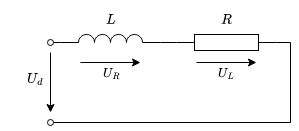
\includegraphics[width=0.5\linewidth]{assets/Chap4/SchemaBobine.png}
    \caption{Schéma électrique simplifié d'une bobine}
\end{figure}

La tension totale correspond à la somme des tensions aux bornes de ces composants, définie par l'équation \ref{eq:TensionBobineEtape1} :

\begin{equation}
    U_d(t) = U_R(t) + U_L(t) = R\cdot i(t) + \frac{d\Psi}{dt} = R\cdot i(t) + \frac{d}{dt}[L(\delta)\cdot i(t)]
    \label{eq:TensionBobineEtape1}
\end{equation}

L'inductance variant en fonction de la position, le développement du terme de dérivation permet d'introduire la vitesse mécanique par substitution dans l'équation \ref{eq:TensionBobineEtape2} :

\begin{equation}
    U_d = R\cdot i + L\cdot \frac{di}{dt} + \frac{dL}{dt} \cdot i = R\cdot i + L\cdot \frac{di}{dt} + \frac{dL}{d\delta}\cdot \frac{d\delta}{dt} \cdot i
    \label{eq:TensionBobineEtape2}
\end{equation}

Afin de déterminer la dérivée de l'inductance par rapport à la position, l'expression simplifiée \ref{eq:IndSimple} est utilisée. Sa dérivation conduit à l'équation \ref{eq:IndDerive} :

\begin{equation}
    \frac{dL(\delta)}{d\delta} = -L_n \cdot \frac{\delta_n}{\delta^2}
    \label{eq:IndDerive}
\end{equation}

En injectant les relations \ref{eq:IndDerive} et \ref{eq:IndSimple} dans l'équation \ref{eq:TensionBobineEtape2}, l'expression \ref{eq:TensionBobineEtape3} est obtenue :

\begin{equation}
    U_d = R \cdot i + L_n \frac{\delta_n}{\delta} \cdot \frac{di}{dt} - i \cdot L_n \frac{\delta_n}{\delta^2} \cdot \dot{\delta}
    \label{eq:TensionBobineEtape3}
\end{equation}

Il est alors possible d'isoler la dérivée temporelle du courant afin d'obtenir l'équation d'état \ref{eq:CourDerive} :

\begin{equation}
    \frac{di}{dt} = \frac{U_d - R \cdot i}{L_n} \cdot \frac{\delta}{\delta_n} + \frac{i}{\delta} \cdot \dot{\delta}
    \label{eq:CourDerive}
\end{equation}

\subsection{Équation de Newton}
L'objectif de ce projet étant d'assurer la lévitation d'une charge mécanique, l'application des lois de la dynamique de Newton est requise. En se basant sur les conventions de la figure \ref{fig:BobineRep}, le principe fondamental de la dynamique s'écrit :

\begin{equation}
    m \cdot \ddot{\delta} =\sum F = F_p - F_{el} = m \cdot g - F_{el}
    \label{eq:Newton1}
\end{equation}

Avec :
\begin{itemize}
    \item $F_p$ : La force de pesanteur [N].
    \item $F_{el}$ : La force électromagnétique [N].
\end{itemize}

La force électromagnétique se déduit de la dérivée de la coénergie magnétique par rapport à la position :
\label{subsec:Fele}

\begin{equation}
    F_{el} =\frac{dW_{mag}}{d\delta}= - \frac{1}{2} \cdot i^2 \cdot \frac{dL(\delta)}{d\delta} = \frac{1}{2} \cdot i^2 \cdot L_n \cdot \frac{\delta_n}{\delta^2}
    \label{eq:Fele}
\end{equation}

À partir de la relation \ref{eq:Fele}, il est possible d'établir l'expression de la force sous sa forme simplifiée :

\begin{equation}
    F_{el} = \frac{1}{2} \cdot i^2 \cdot L_n \cdot \frac{\delta_n}{\delta^2} = i^2 \cdot k \cdot \frac{1}{\delta^2}
    \label{eq:MethInv1}
\end{equation}

Avec la constante $k$ définie par :

\begin{equation}
    k = \frac{L_n\cdot\delta_n}{2} = \frac{4,9\cdot 10^{-3}\cdot 2\cdot 10^{-3}}{2}=4,9\cdot 10^{-6} \text{ } \text{N}\cdot\text{m}^2/\text{A}^2
\end{equation}

La méthode inverse, implémentée au sein du microcontrôleur, consiste à isoler le courant requis à partir de l'équation \ref{eq:MethInv1} :

\begin{equation}
    i = \sqrt{\frac{F_{el}}{k}} \cdot \delta
    \label{eq:MethInv2}
\end{equation}

L'équation \ref{eq:MethInv2} sera principalement employée dans le code source ainsi que pour le calcul des différents paramètres lors de l'étape de linéarisation \ref{subsec:lin}.

L'introduction de la relation \ref{eq:Fele} dans l'équation mécanique \ref{eq:Newton1} conduit à l'expression \ref{eq:Newton2} :

\begin{equation}
    m \cdot \ddot{\delta} = m\cdot g - \frac{1}{2} \cdot i^2 \cdot L_n \cdot \frac{\delta_n}{\delta^2}
    \label{eq:Newton2}
\end{equation}

Enfin, l'isolation du terme d'accélération permet d'obtenir l'équation différentielle finale :

\begin{equation}
    \frac{d^2\delta}{dt^2} = g - \frac{L_n \cdot \delta_n}{2 \cdot m} \cdot \left(\frac{i}{\delta}\right)^2
    \label{eq:Accel}
\end{equation}

\subsection{Linéarisation des équations}
\label{subsec:lin}
Le système présente un comportement fortement non linéaire, comme l'illustrent les équations \ref{eq:CourDerive} et \ref{eq:Accel}. Il est donc nécessaire de linéariser ces expressions afin de permettre le réglage du système. À cette fin, une linéarisation est réalisée par la méthode du développement en série de Taylor.\\

Les équations à linéariser sont définies par le système suivant :

\begin{equation*}
    \left\{ \begin{aligned}
         & f_1(i, \delta, \dot{\delta}, U_{d}) = \frac{di}{dt} = \frac{U_d - R \cdot i}{L_n} \cdot \frac{\delta}{\delta_n} + \frac{i}{\delta} \cdot \dot{\delta} \\
         & f_2(i, \delta) = \frac{d^2\delta}{dt^2} = g - \frac{L_n \cdot \delta_n}{2 \cdot m} \cdot \left(\frac{i}{\delta}\right)^2
    \end{aligned} \right.
\end{equation*}

Il est crucial de définir préalablement un point de fonctionnement nominal. La consigne du système étant fixée à 2~mm, cette valeur est choisie comme référence nominale. Par conséquent, les différentes grandeurs associées à ce point de fonctionnement sont :

\begin{itemize}
    \item La position nominale $\delta_n$ vaut 2~mm.
    \item La vitesse et l'accélération au point nominal sont nulles ($\dot{\delta}_n = \ddot{\delta}_n = 0$).
    \item Le courant nominal traversant les bobines est noté $i_n$.
    \item La variation temporelle du courant est nulle ($\frac{di}{dt} = 0$).
    \item La tension nominale appliquée aux bobines est notée $U_{d,n}$.
\end{itemize}

Ces considérations permettent de calculer le courant et la tension au point de fonctionnement nominal.\\

L'accélération étant nulle au point fixe, la force électromagnétique doit compenser exactement la force de pesanteur afin de maintenir la maquette en lévitation :

$$m\cdot\ddot{\delta} = F_p - F_{el} = 0$$

\begin{equation}
    F_{el} = F_p = m\cdot g = 4,513 \cdot 9,81 = 44,3 \text{ N}
\end{equation}

En appliquant la relation \ref{eq:MethInv2} aux grandeurs nominales, le courant nominal est déterminé par :

\begin{equation}
    i_n = \sqrt{\frac{F_{el}}{k}}\cdot\delta_n = \sqrt{\frac{44,3}{4,9\cdot 10^{-6}}}\cdot 2\cdot 10^{-3} = 6,01 \text{ A}
\end{equation}

La tension nominale se déduit de l'équation \ref{eq:TensionBobineEtape2}. La variation de courant et la vitesse mécanique étant nulles, seul le comportement résistif de l'enroulement subsiste. La tension nominale se calcule alors par la loi d'Ohm :

\begin{equation}
    U_{d,n} = R\cdot i_n = 0,8 \cdot 6,01 = 4,81 \text{ V}
\end{equation}

Le développement en série de Taylor peut dès lors être appliqué. Pour alléger les notations, l'indice $n$ au niveau des barres d'évaluation indique que l'expression est évaluée au point de fonctionnement nominal.\\

La fonction $f_1$ dépend de quatre variables et se linéarise selon l'expression suivante :

\begin{equation}
    f_1(i, \delta, \dot{\delta}, U_d) \approx f_1(n)
    + \left. \frac{\partial f_1}{\partial i} \right|_{n}\cdot\Delta{i}
    + \left. \frac{\partial f_1}{\partial \delta} \right|_{n}\cdot\Delta{\delta}
    + \left. \frac{\partial f_1}{\partial \dot{\delta}} \right|_{n}\cdot\Delta{\dot{\delta}}
    + \left. \frac{\partial f_1}{\partial U_d} \right|_{n}\cdot\Delta{U_d}
    \label{eq:f1Lin1}
\end{equation}

Avec les définitions suivantes :

\begin{equation}
    \Delta i = i-i_n \qquad \Delta\delta = \delta-\delta_n \qquad \Delta\dot{\delta} = \dot{\delta}-\overset{=0}{\cancel{\dot{\delta}_n}} = \dot{\delta} \qquad \Delta U_d = U_d-U_{d,n}
    \label{eq:DeltaDef}
\end{equation}

Les évaluations des dérivées partielles au point nominal donnent :

\begin{equation}
    f_1(n)  = \frac{\overset{=0}{\cancel{U_{d,n} - R \cdot i_n}}}{L_n} \cdot \frac{\delta_n}{\delta_n} + \frac{i_n}{\delta_n} \cdot \overset{=0}{\cancel{\dot{\delta}_n}} = 0
    \label{eq:DerivePart1}
\end{equation}

\begin{equation}
    \left. \frac{\partial f_1}{\partial i} \right|_{n} = \left. \left(-\frac{R}{L_n}\cdot\frac{\delta}{\delta_n}+\frac{\dot{\delta}}{\delta}\right) \right|_{n} = -\frac{R}{L_n}\cdot\frac{\delta_n}{\delta_n}+0 = -\frac{R}{L_n}
    \label{eq:DerivePart2}
\end{equation}

\begin{equation}
    \left. \frac{\partial f_1}{\partial \delta} \right|_{n} = \left. \left( \frac{U_d - R\cdot i}{L_n \cdot \delta_n} - \frac{i \cdot \dot{\delta}}{\delta^2} \right) \right|_{n} = \frac{\overset{=0}{\cancel{U_{d,n} - R\cdot i_n}}}{L_n \cdot \delta_n} - 0 = 0
    \label{eq:DerivePart3}
\end{equation}

\begin{equation}
    \left. \frac{\partial f_1}{\partial \dot{\delta}} \right|_{n} = \left. \left( \frac{i}{\delta} \right) \right|_{n} = \frac{i_n}{\delta_n}
    \label{eq:DerivePart4}
\end{equation}

\begin{equation}
    \left. \frac{\partial f_1}{\partial U_d} \right|_{n} =
    \left. \left( \frac{1}{L_n}\cdot\frac{\delta}{\delta_n} \right) \right|_{n} = \frac{1}{L_n}\cdot\frac{\delta_n}{\delta_n} = \frac{1}{L_n}
    \label{eq:DerivePart5}
\end{equation}

En substituant les équations \ref{eq:DeltaDef} à \ref{eq:DerivePart5} dans la relation \ref{eq:f1Lin1}, il vient :

$$f_1(i, \delta, \dot{\delta}, U_d) \approx
    -\frac{R}{L_n} \cdot (i-i_n)
    + 0 \cdot (\delta-\delta_n)
    + \frac{i_n}{\delta_n}\cdot\dot{\delta}
    + \frac{1}{L_n}\cdot (U_d-U_{d,n}) $$

$$f_1(i, \delta, \dot{\delta}, U_d) \approx
    -\frac{R}{L_n} \cdot (i-i_n)
    + \frac{i_n}{\delta_n}\cdot\dot{\delta}
    + \frac{1}{L_n}\cdot (U_d-R\cdot i_n)$$

$$f_1(i, \delta, \dot{\delta}, U_d) \approx
    -\frac{R}{L_n} \cdot i
    + \cancel{\frac{R}{L_n} \cdot i_n}
    + \frac{i_n}{\delta_n}\cdot\dot{\delta}
    + \frac{1}{L_n}\cdot U_d
    - \cancel{\frac{R}{L_n}\cdot i_n} $$

\begin{equation}
    f_1(i, \delta, \dot{\delta}, U_d) = \frac{di}{dt} \approx
    -\frac{R}{L_n} \cdot i
    + \frac{i_n}{\delta_n}\cdot\dot{\delta}
    + \frac{1}{L_n}\cdot U_d
    \label{eq:f1Lin2}
\end{equation}

La fonction $f_2$ se linéarise de la même manière :

\begin{equation}
    f_2(i, \delta) \approx f_2(n)
    + \left. \frac{\partial f_2}{\partial i} \right|_{n}\cdot\Delta{i}
    + \left. \frac{\partial f_2}{\partial \delta} \right|_{n}\cdot\Delta{\delta}
    \label{eq:f2Lin1}
\end{equation}

Avec :

\begin{equation}
    \Delta i = i-i_n \qquad
    \Delta\delta = \delta-\delta_n
    \label{eq:DeltaDef2}
\end{equation}

\begin{equation}
    f_2(n) = \ddot{\delta}_n = 0
    \label{eq:DerivePart6}
\end{equation}

\begin{equation}
    \left. \frac{\partial f_2}{\partial i} \right|_{n} = \left. \left( 0 - \frac{1}{\cancel{2}\cdot m}\cdot \cancel{2}\cdot i\cdot L_n \cdot\delta_n\cdot\frac{1}{\delta^2}\right) \right|_{n} = -\frac{i_n\cdot L_n}{m \cdot\delta_n}
    \label{eq:DerivePart7}
\end{equation}

\begin{equation}
    \left. \frac{\partial f_2}{\partial \delta} \right|_{n} = \left. \left( 0 - \frac{1}{2\cdot m}\cdot i^2\cdot L_n \cdot\delta_n\cdot\frac{-2}{\delta^3}\right) \right|_{n} = \frac{i_n^2\cdot L_n \cdot \delta_n}{m \cdot\delta_n^3}= \frac{i_n^2\cdot L_n}{m \cdot\delta_n^2}
    \label{eq:DerivePart8}
\end{equation}

En injectant les expressions \ref{eq:DeltaDef2} à \ref{eq:DerivePart8} dans la relation \ref{eq:f2Lin1}, on obtient :

$$    f_2(i, \delta) = \frac{d^2\delta}{dt^2} \approx
    -\frac{i_n\cdot L_n}{m \cdot\delta_n}\cdot(i-i_n)
    + \frac{i_n^2\cdot L_n}{m \cdot\delta_n^2}\cdot(\delta-\delta_n)$$

$$    f_2(i, \delta) = \frac{d^2\delta}{dt^2} \approx
    -\frac{i_n\cdot L_n}{m \cdot\delta_n}\cdot i
    +\cancel{\frac{i_n^2\cdot L_n}{m \cdot\delta_n}}
    + \frac{i_n^2\cdot L_n}{m \cdot\delta_n^2}\cdot\delta
    -\cancel{\frac{i_n^2\cdot L_n}{m \cdot\delta_n}}$$

\begin{equation}
    f_2(i, \delta) = \frac{d^2\delta}{dt^2} \approx
    -\frac{i_n\cdot L_n}{m \cdot\delta_n}\cdot i
    + \frac{i_n^2\cdot L_n}{m \cdot\delta_n^2}\cdot\delta
    \label{eq:f2Lin2}
\end{equation}

\section{La régulation de courant}

La régulation de courant est synthétisée au moyen d'un régulateur PI. Le schéma bloc de la figure \ref{fig:SchemaBlocRegCur} représente cette architecture :

\begin{figure}[H]
    \centering
    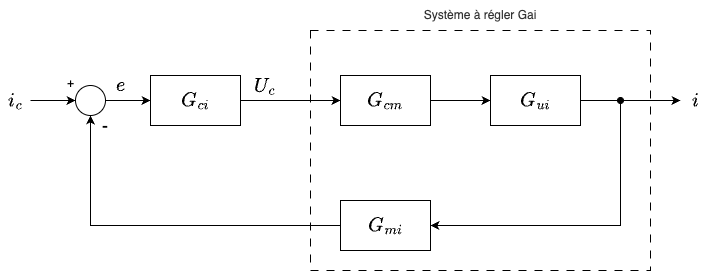
\includegraphics[width=0.75\linewidth]{assets/Chap4/RegulCourBloc.png}
    \caption{Schéma bloc de la régulation de courant par un PI}
    \label{fig:SchemaBlocRegCur}
\end{figure}

Le développement du modèle s'appuie sur la mise en commun des équations linéarisées précédemment :

\begin{equation*}
    \left\{ \begin{aligned}
         & \frac{di}{dt} \approx
        -\frac{R}{L_n} \cdot i
        + \frac{i_n}{\delta_n}\cdot\dot{\delta}
        + \frac{1}{L_n}\cdot U_d          \\
         & \frac{d^2\delta}{dt^2} \approx
        -\frac{i_n\cdot L_n}{m \cdot\delta_n}\cdot i
        + \frac{i_n^2\cdot L_n}{m \cdot\delta_n^2}\cdot\delta
    \end{aligned} \right.
\end{equation*}

Comme décrit dans le rapport de Laucella \cite{Laucella}, une analogie peut être établie avec le moteur à courant continu. L'équation mécanique régissant une telle machine définit l'accélération angulaire $\frac{d\Omega}{dt}$ (où $\Omega$ représente la vitesse angulaire) en fonction du courant $i$ et d'un couple de frottement résistant $C_r$, ce dernier pouvant être négligé :

$$J \cdot \frac{d\Omega}{dt} = \sum T = T_{em} - T_{frott}$$

$$\frac{d\Omega}{dt} = \frac{T_{em}}{J} - \frac{T_{frott}}{J}$$

\begin{equation}
    \frac{d\Omega}{dt} = \frac{K_T}{J}\cdot i - \frac{C_r}{J}
\end{equation}

Dans ce modèle, l'accélération est indépendante de la position angulaire du rotor. En appliquant ce même principe au système de sustentation, il est possible de supposer, par comparaison des deux dynamiques, que l'influence de la position peut être omise. L'équation mécanique linéarisée complète s'écrit :

\begin{equation*}
    \frac{d^2\delta}{dt^2} \approx
    -\frac{i_n\cdot L_n}{m \cdot\delta_n}\cdot i
    + \frac{i_n^2\cdot L_n}{m \cdot\delta_n^2}\cdot\delta
\end{equation*}

Par conséquent, la composante liée à la position ($\delta$) est négligée afin de rapprocher le comportement du système de celui d'un moteur électrique et de simplifier la régulation de courant. Le système d'équations se réduit à la forme suivante :

\begin{equation*}
    \left\{ \begin{aligned}
         & \frac{di}{dt} \approx -\frac{R}{L_n} \cdot i + \frac{i_n}{\delta_n}\cdot\dot{\delta} + \frac{1}{L_n}\cdot U_d \\
         & \frac{d^2\delta}{dt^2} \approx -\frac{i_n\cdot L_n}{m \cdot\delta_n}\cdot i
    \end{aligned} \right.
\end{equation*}

Une simulation a été réalisée par Laucella \cite{Laucella}, prouvant l'efficacité du système avec et sans cette simplification :

\begin{figure}[H]
    \centering
    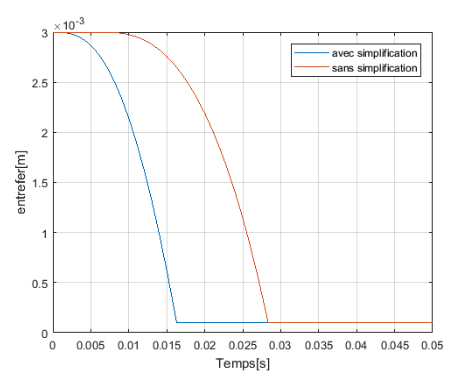
\includegraphics[width=0.75\linewidth]{assets/Chap4/ModélisationDeSimplification.png}
    \caption{Vérification de la simplification de l'accélération \cite{Laucella}}
\end{figure}

Pour insérer l'équation de l'accélération dans celle de la variation de courant, la variation du courant est dérivée une fois supplémentaire par rapport au temps :

\begin{equation*}
    \left\{ \begin{aligned}
         & \frac{d^2i}{dt^2} = -\frac{R}{L_n} \cdot \frac{di}{dt} + \frac{i_n}{\delta_n}\cdot\frac{d^2\delta}{dt^2} + \frac{1}{L_n}\cdot \frac{dU_d}{dt} \\
         & \frac{d^2\delta}{dt^2} = -\frac{i_n\cdot L_n}{m \cdot\delta_n}\cdot i
    \end{aligned} \right.
\end{equation*}

En substituant l'accélération mécanique dans la dynamique du courant, l'expression différentielle globale est obtenue :

$$    \frac{d^2i}{dt^2} = -\frac{R}{L_n} \cdot \frac{di}{dt} - \frac{i_n}{\delta_n}\cdot\frac{i_n\cdot L_n}{m \cdot\delta_n}\cdot i + \frac{1}{L_n}\cdot \frac{dU_d}{dt}$$

\begin{equation}
    \frac{d^2i}{dt^2} = -\frac{R}{L_n} \cdot \frac{di}{dt} - \frac{i_n^2\cdot L_n}{m \cdot\delta_n^2}\cdot i + \frac{1}{L_n}\cdot \frac{dU_d}{dt}
    \label{eq:FinalEq1}
\end{equation}

En appliquant la transformée de Laplace à l'équation \ref{eq:FinalEq1}, la fonction de transfert correspondante est déterminée :

$$ s^2\cdot I(s) = -\frac{R}{L_n} \cdot s\cdot I(s) - \frac{i_n^2\cdot L_n}{m \cdot\delta_n^2}\cdot I(s) + \frac{1}{L_n}\cdot s\cdot U_d(s) $$

$$ I(s)\cdot \left( s^2 + \frac{R}{L_n} \cdot s + \frac{i_n^2\cdot L_n}{m \cdot\delta_n^2}\right) = \frac{1}{L_n}\cdot s\cdot U_d(s) $$

$$ G_{ui}(s) = \frac{I(s)}{U_d(s)} = \frac{s}{L_n\cdot \left( s^2 + \frac{R}{L_n} \cdot s + \frac{i_n^2\cdot L_n}{m \cdot\delta_n^2}\right)}$$

$$ G_{ui}(s) = \frac{I(s)}{U_d(s)} = \frac{s}{L_n\cdot\frac{i_n^2\cdot L_n}{m \cdot\delta_n^2}\cdot\left(\frac{m\cdot\delta_n^2}{i_n^2\cdot L_n}\cdot s^2 + \frac{m\cdot\delta_n^2}{i_n^2\cdot \cancel{L_n}}\cdot\frac{R}{\cancel{L_n}} \cdot s + 1 \right)}$$

$$ G_{ui}(s) = \frac{I(s)}{U_d(s)} = \frac{m \cdot\delta_n^2}{i_n^2\cdot L_n^2}\cdot\frac{s}{ \frac{m\cdot\delta_n^2}{i_n^2\cdot L_n}\cdot s^2 + \frac{m\cdot\delta_n^2\cdot R}{i_n^2\cdot L_n^2} \cdot s + 1}$$

\begin{equation}
    G_{ui}(s) = \frac{I(s)}{U_d(s)} = K_{ui}\cdot\frac{s}{1 + a_1 \cdot s + a_2\cdot s^2}
\end{equation}

Avec :

\begin{equation*}
    \left\{ \begin{aligned}
         & K_{ui} = \frac{m}{L_n^2}\cdot \left(\frac{\delta_n}{i_n} \right)^2                     \\
         & a_1 = \frac{m\cdot R}{L_n^2}\cdot \left(\frac{\delta_n}{i_n} \right)^2                 \\
         & a_2 = \frac{m}{L_n}\cdot\left(\frac{\delta_n}{i_n^2}\right)^2 = \frac{L_n}{R}\cdot a_1
    \end{aligned} \right.
\end{equation*}

Ceci est la fonction de transfert avec la simplification, sans celle-ci le résultat fut calculer dans le travail de bachelor de Laucella \cite{Laucella} donnat alors l'équation suivante :

\begin{equation}
    G_{ui}(s) = K_{ui}\cdot\frac{1-a_1 \cdot s^2}{1 - a_1 \cdot s^2 - a_2\cdot s^3}
\end{equation}

Avec :

\begin{equation*}
    \left\{ \begin{aligned}
         & K_{ui} = \frac{1}{R}                                          \\
         & a_1 = \frac{m}{L_n}\cdot \left(\frac{\delta_n}{i_n} \right)^2 \\
         & a_2 = \frac{L_n}{R}\cdot a_1
    \end{aligned} \right.
\end{equation*}

Une comparaison fut dès alors réaliser par Laucella \cite{Laucella} donnant ainsi la \autoref{} :

\begin{figure}[H]
    \centering
    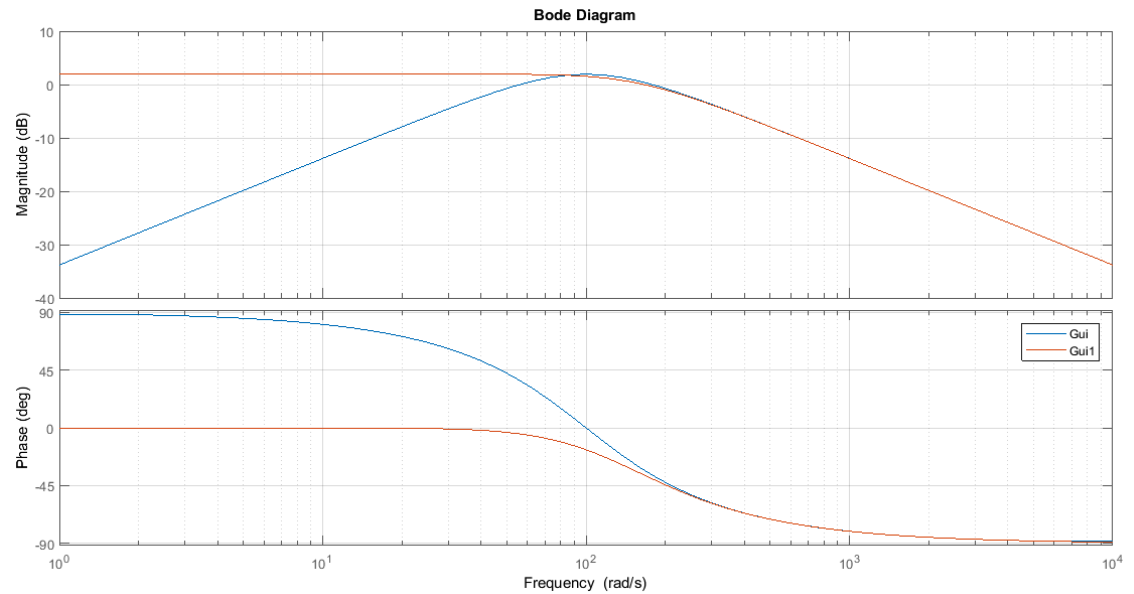
\includegraphics[width=1\linewidth]{assets/Chap4/CompSimpleEtBrute.png}
    \caption{Comparaison entre l'équation simplifié et l'équation brute \cite{Laucella}}
\end{figure}

Avec $G_{ui}$ l'équation simplifié et $G_{ui1}$ l'équation brute.

L'analyse du système démontre qu'en basse fréquence, l'action dérivateur est bien dominante sur l'équation $G_{ui1}$. La droite commençant à 90°. Les deux courbes viennent se supperposer vers les aléantour de 100 rad/s. Dès lors les traces sont presque identique. Il est alors acceptable d'admettre que la simplification est possible car le résultat final dépendra principalement des sommes des petites constantes de temps qui viennent agir sur des fréquence plus élevé.

Le bloc $G_{cm}$, représentant l'organe de commande, est approximé par un filtre passe-bas du premier ordre :

\begin{equation}
    G_{cm} = \frac{K_{cm}}{1+s \cdot\tau_{cm}} = \frac{1}{1+s \cdot\tau_{cm}}
\end{equation}

La maquette met en œuvre une modulation PWM numérique. Celle-ci dicte la constante de temps de l'organe de commande $\tau_{cm}$, qui correspond à la période d'échantillonnage :

\begin{equation}
    \tau_{cm} = h = 40 \text{ $\mu$s}
\end{equation}

L'organe de mesure du courant $G_{mi}$ est également approximé par un filtre passe-bas du premier ordre :

\begin{equation}
    G_{mi} = \frac{K_{mi}}{1+s \cdot\tau_{mi}} = \frac{1}{1+s \cdot\tau_{mi}}
\end{equation}

La constante de temps du capteur est déterminée à partir de la fiche technique du fabricant \cite{CaptCour}, qui indique une bande passante de 50~kHz. Afin de respecter le critère de Shannon \cite{Shanon}, la fréquence de coupure du filtre anti-repliement a été fixée à 25~kHz, ce qui correspond à la fréquence d'échantillonnage du DSP :

\begin{equation}
    \tau_{mi} = \frac{1}{f_{mi}} = \frac{1}{25\cdot 10^3} = 6.4 \text{ $\mu$s}
\end{equation}

La fonction de transfert du système à régler s'écrit alors :

\begin{equation}
    G_{ai} = G_{ui} \cdot G_{cm} \cdot G_{mi} = K_{ui}\cdot\frac{s}{1 + a_1 \cdot s + a_2\cdot s^2} \cdot \frac{1}{1+s \cdot\tau_{cm}} \cdot \frac{1}{1+s \cdot\tau_{mi}}
\end{equation}

Une fois cette fonction implémentée dans Matlab, le diagramme de Bode peut être tracé.

\begin{figure}[H]
    \centering
    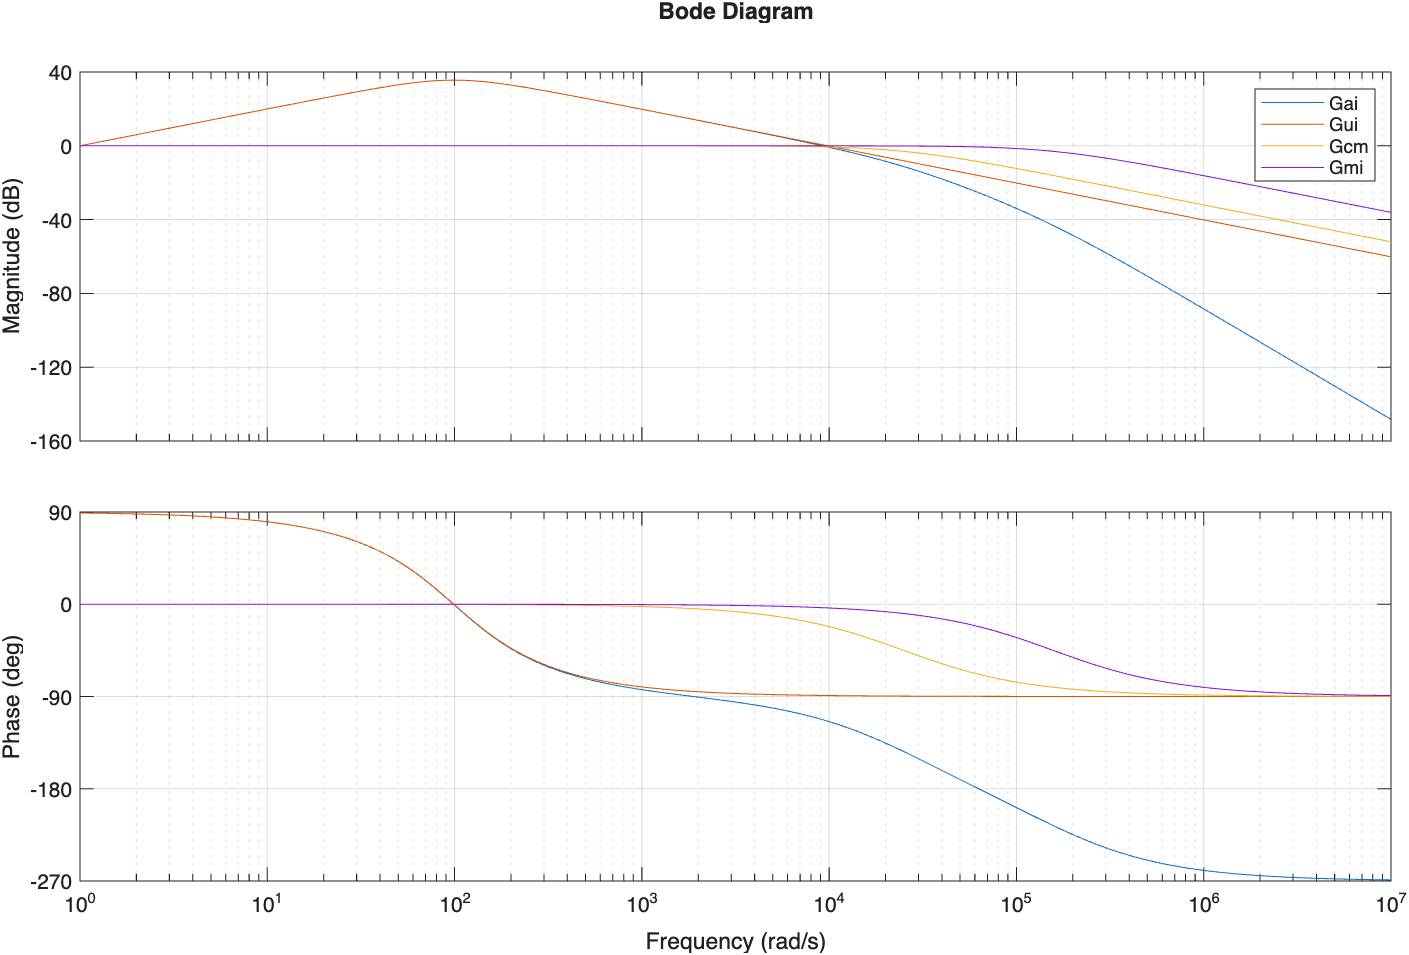
\includegraphics[width=1\linewidth]{assets/Chap4/BodeGaiFaux.png}
    \caption{Diagramme de bode du système à régler}
\end{figure}

La fonction de transfert du régulateur est donnée par l'équation \ref{eq:PI} :

\begin{equation}
    G_{ci} = K_{pi}\cdot\frac{1+s\cdot\tau_{ii}}{s\cdot\tau_{ii}}
    \label{eq:PI}
\end{equation}

Le système en boucle ouverte $G_{BO}$ est défini par la relation suivante :

$$G_{BO} = G_{ci}\cdot G_{ai}$$

\begin{equation}
    G_{BO} = K_{pi}\cdot\frac{1+s\cdot\tau_{ii}}{s\cdot\tau_{ii}}\cdot K_{ui}\cdot\frac{s}{1 + a_1 \cdot s + a_2\cdot s^2} \cdot \frac{1}{1+s \cdot\tau_{cm}} \cdot \frac{1}{1+s \cdot\tau_{mi}}
\end{equation}

Il convient de déterminer la constante de temps du régulateur $\tau_{ii}$ ainsi que son gain $K_{pi}$.\\

La constante de temps se définit comme le produit de la somme des petites constantes de temps par un coefficient $N$. Les petites constantes de temps correspondent à $\tau_{cm}$ et $\tau_{mi}$ :

\begin{equation}
    \tau_{ii} = N \cdot\sum\tau_{pct} = N \cdot \left(\tau_{cm} + \tau_{mi}\right) = N \cdot \left(40 + 6.4\right)\cdot 10^{-6} = N \cdot 46.4\cdot 10^{-6}
\end{equation}

Afin de déterminer une valeur adéquate pour $N$, une analyse paramétrique a été effectuée pour des valeurs de $N$ comprises entre 5 et 15. La bande passante et l'erreur ont été évaluées pour établir un compromis optimal entre la précision statique et la rapidité du système. Les résultats sont observables de la figure \ref{fig:DiffN} à la figure \ref{fig:Erreur} :

\begin{figure}[H]
    \centering
    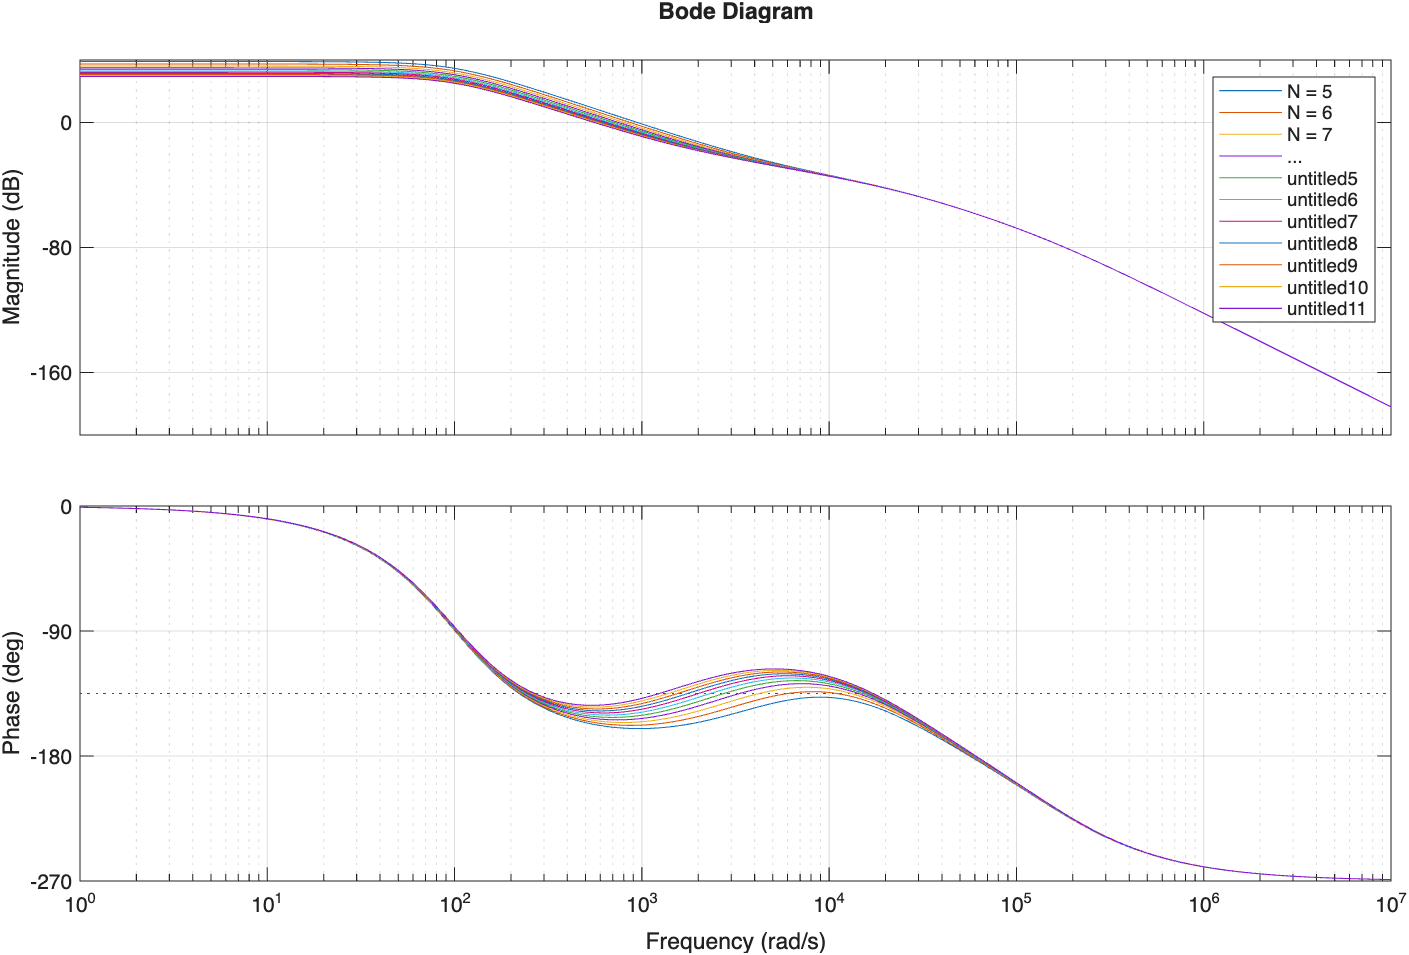
\includegraphics[width=1\linewidth]{assets/Chap4/TraceN.png}
    \caption{Réponse fréquentielle du système réglé pour différentes valeurs de $N$}
    \label{fig:DiffN}
\end{figure}

\begin{figure}[H]
    \centering
    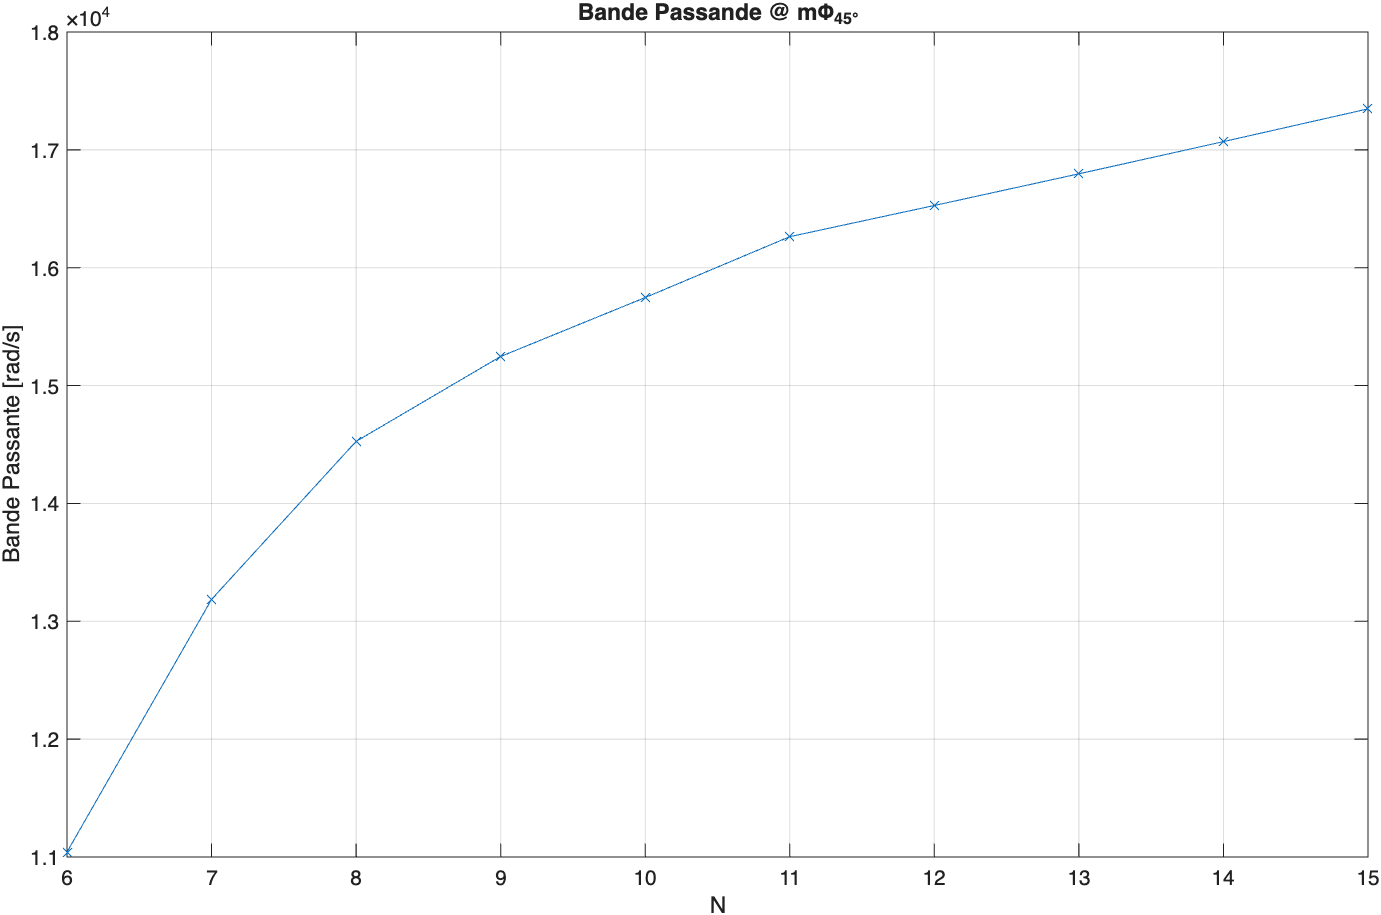
\includegraphics[width=1\linewidth]{assets/Chap4/BP.png}
    \caption{Évolution de la bande passante en fonction de $N$}
    \label{fig:BP}
\end{figure}

\begin{figure}[H]
    \centering
    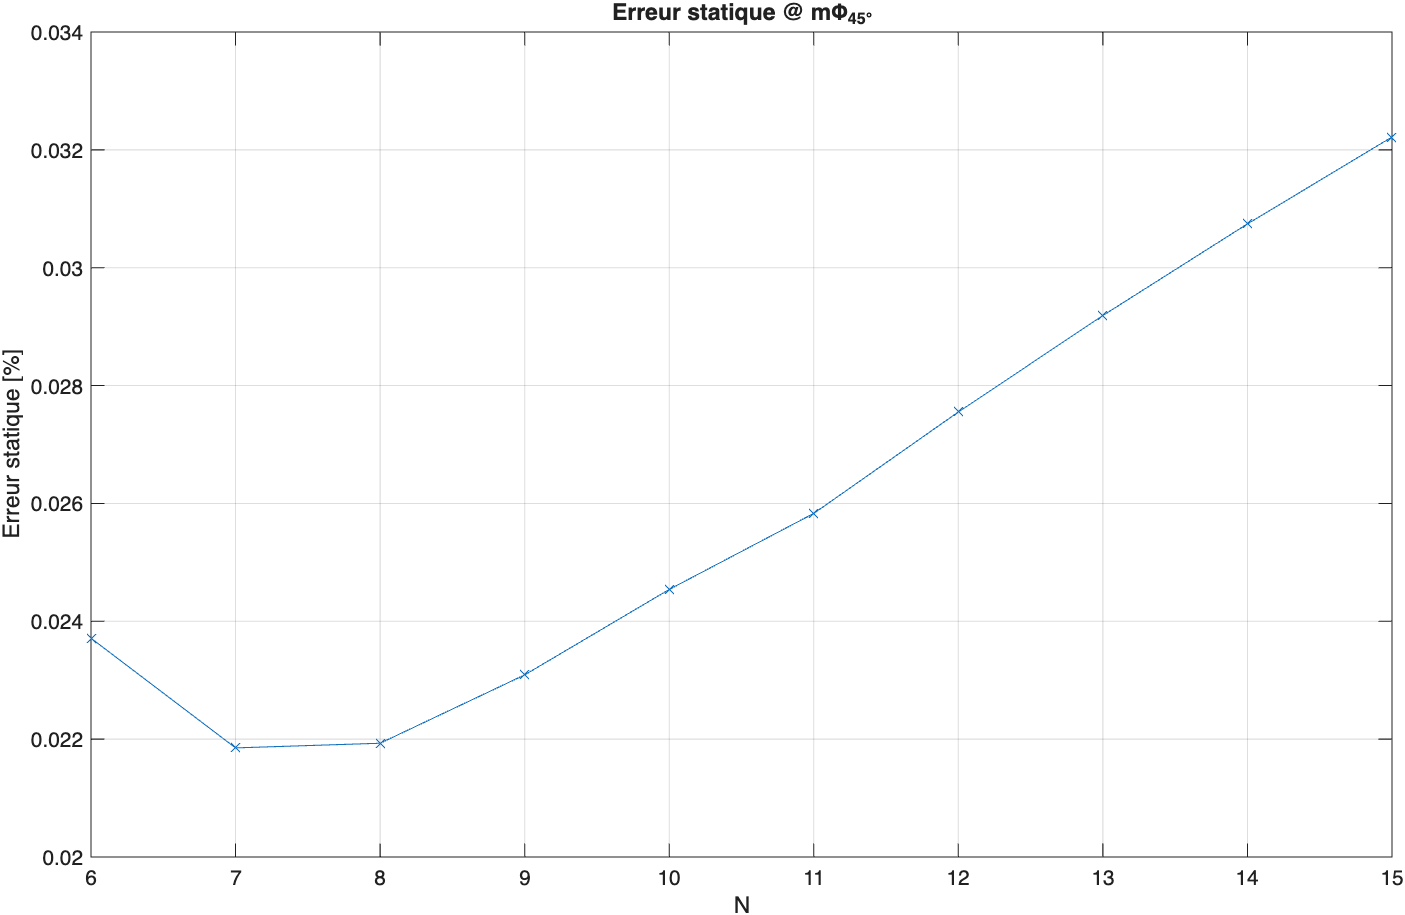
\includegraphics[width=1\linewidth]{assets/Chap4/Erreur.png}
    \caption{Évolution de l'erreur en fonction de $N$}
    \label{fig:Erreur}
\end{figure}

La valeur sélectionnée est $N=10$, ce qui conduit à la constante de temps suivante :

\begin{equation}
    \tau_{ii} = 10 \cdot 46.4 \cdot 10^{-6} = 464 \text{ $\mu$s}
\end{equation}

À partir de cette configuration, le gain $K_{pi}$ est déterminé pour assurer une marge de phase de 45° :

\begin{figure}[H]
    \centering
    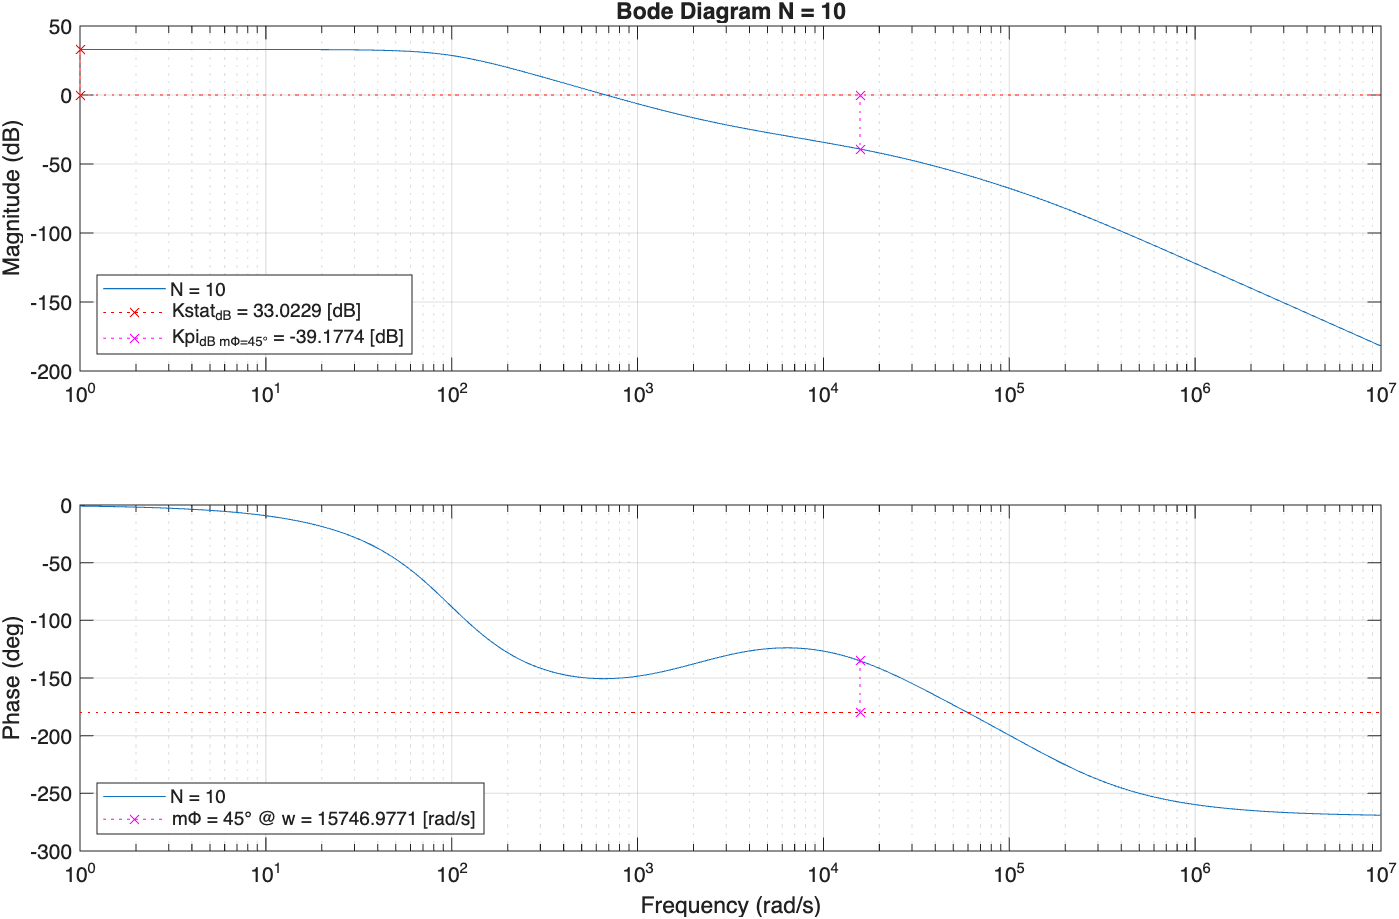
\includegraphics[width=1\linewidth]{assets/Chap4/Kpi45.png}
    \caption{Détermination du gain $K_{pi}$ pour une marge de phase de 45°}
\end{figure}

La valeur de $K_{pi}$ retenue est d'environ 39~dB, ce qui correspond à un gain linéaire de 90.96.

La validation du comportement global est effectuée par l'application d'un saut unitaire en boucle fermée :

\begin{figure}[H]
    \centering
    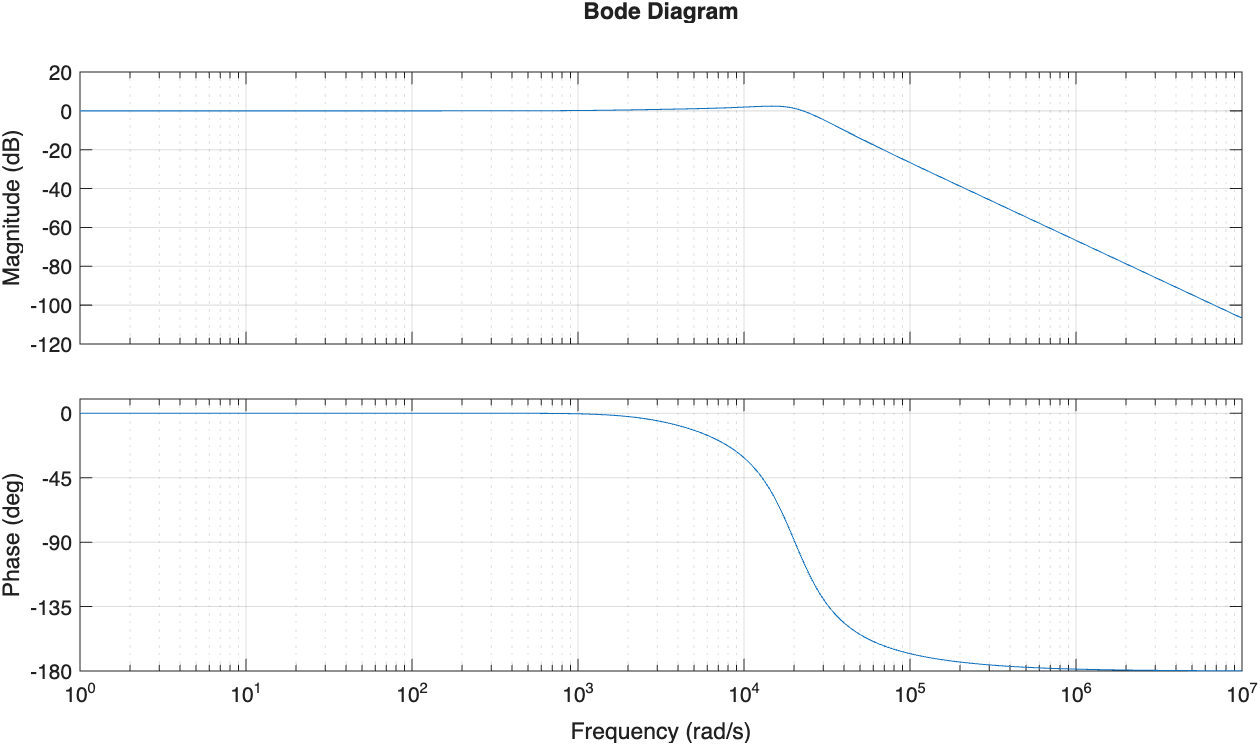
\includegraphics[width=1\linewidth]{assets/Chap4/BF1.png}
    \caption{Réponse fréquentielle en boucle fermée}
\end{figure}

La réponse indicielle de la boucle fermée présente le profil suivant :

\begin{figure}[H]
    \centering
    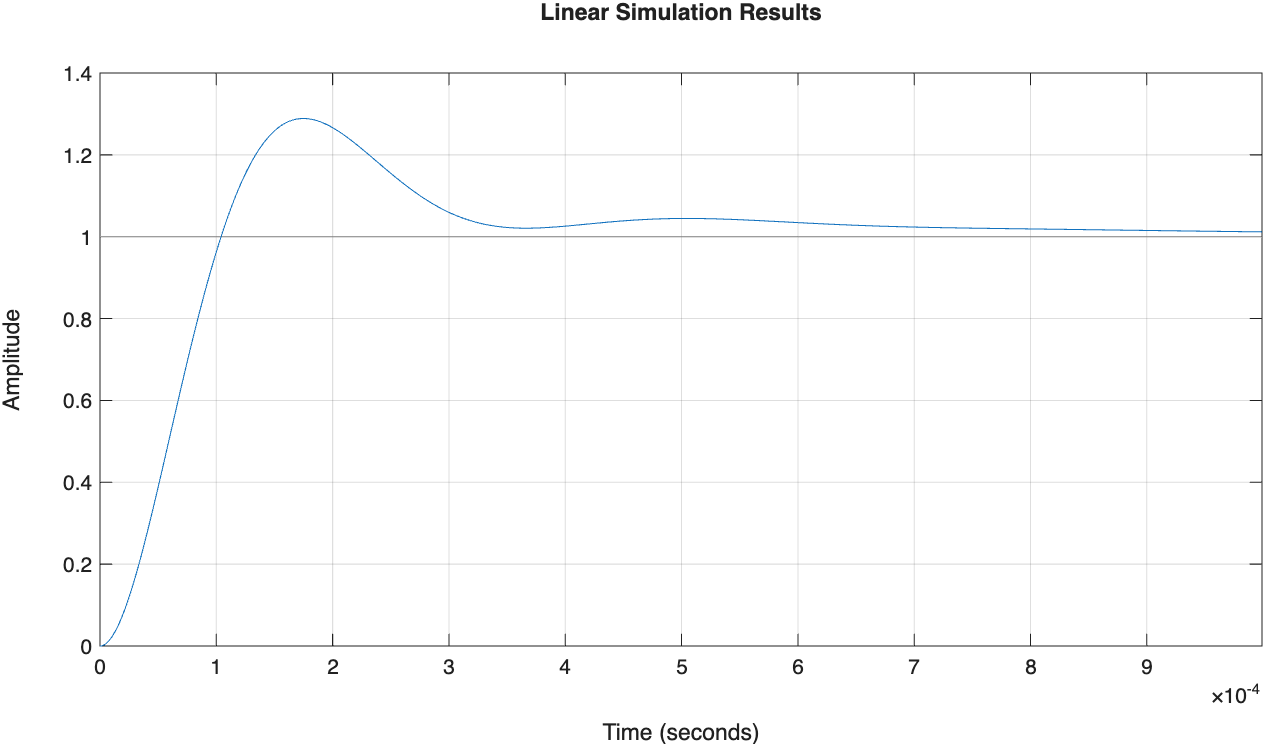
\includegraphics[width=1\linewidth]{assets/Chap4/Step.png}
    \caption{Réponse indicielle de la régulation de courant}
\end{figure}

Les performances de la boucle de courant sont ainsi validées.\\

Enfin, une approximation de ce système par un modèle du premier ordre est réalisée afin de simplifier la future synthèse de la régulation de position. La constante de temps équivalente en boucle fermée est évaluée à la pulsation correspondant à un déphasage de -45°, comme l'illustre la figure \ref{fig:BFPI} :

\begin{figure}[H]
    \centering
    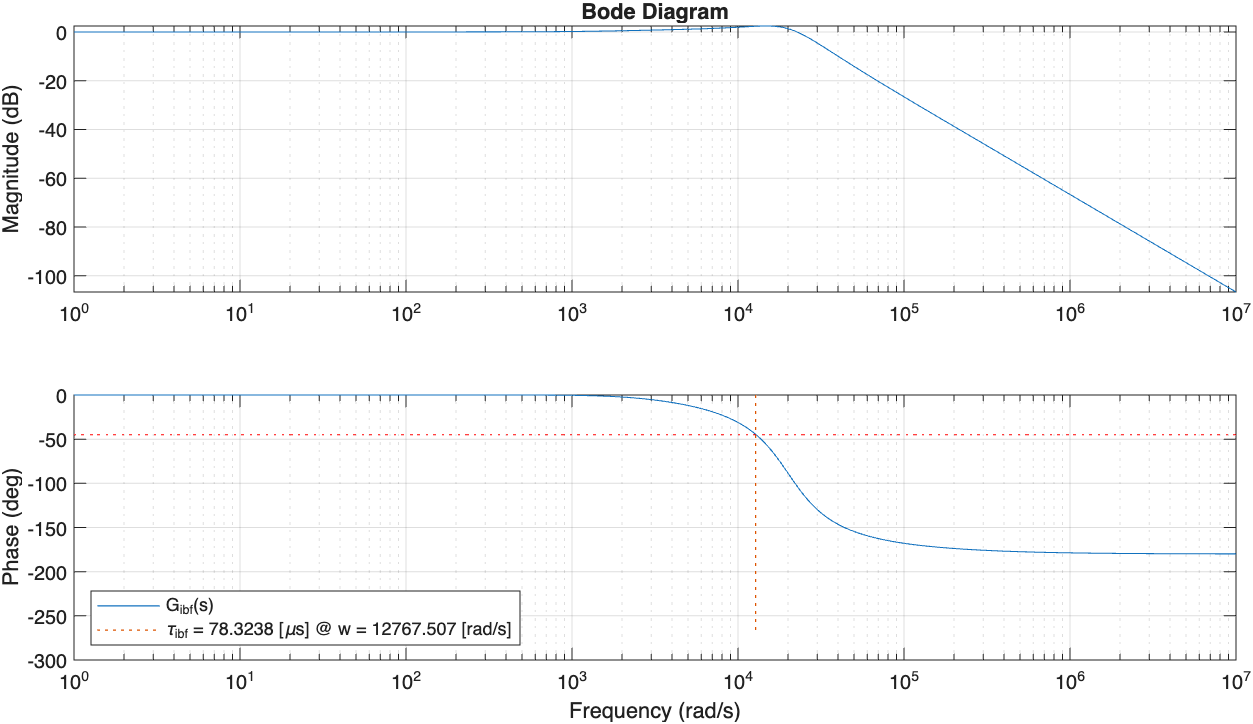
\includegraphics[width=1\linewidth]{assets/Chap4/BF.png}
    \caption{Identification de la constante de temps de la boucle fermée}
    \label{fig:BFPI}
\end{figure}

La constante de temps de la boucle fermée $\tau_{iBF}$ obtenue est de 78,32~$\mu$s.

\begin{figure}[H]
    \centering
    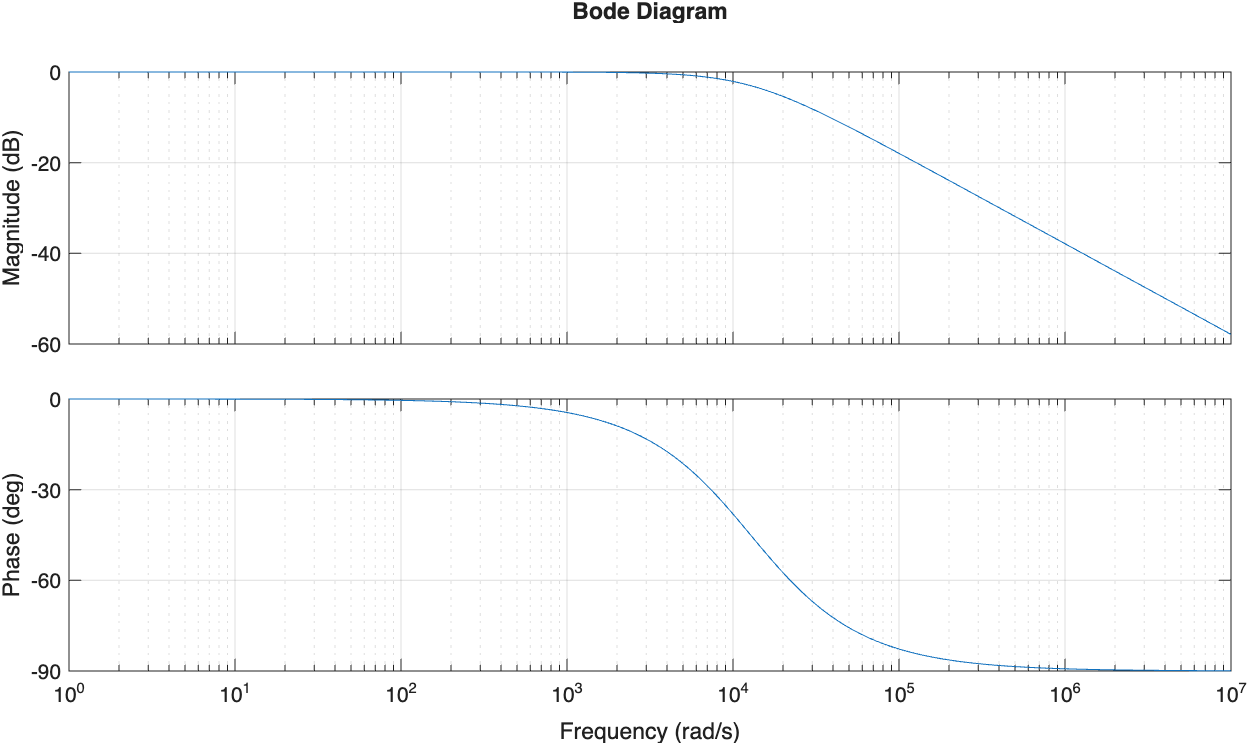
\includegraphics[width=1\linewidth]{assets/Chap4/ApproxPI.png}
    \caption{Diagramme de Bode de l'approximation de la boucle fermée}
\end{figure}

Une comparaison des paramètres du système synthétisé avec et sans la prise en compte de la constante $K_{ui}$ est présentée ci-dessous.

\begin{table}[H]
    \centering
    \begin{tabular}{lcc}
        \hline
        \textbf{Paramètre} & \textbf{Sans $K_{ui}$} & \textbf{Avec $K_{ui}$} \\ \hline
        $\tau_{ii}$        & $4,63 \cdot 10^{-4}$   & $4,63 \cdot 10^{-4}$   \\
        $K_{pi}$           & $1,89$                 & $90,96$                \\
        $\tau_{iBF}$       & $7,83 \cdot 10^{-5}$   & $7,83 \cdot 10^{-5}$   \\ \hline
    \end{tabular}
    \caption{Comparaison des paramètres avec et sans intégration de $K_{ui}$}
    \label{tab:comparatif_kui}
\end{table}

L'analyse de ces données montre que seule la valeur du gain $K_{pi}$ est modifiée. L'introduction d'une constante n'exerce aucune influence sur la phase du système, son déphasage propre étant nul. Ce comportement est confirmé par les figures \ref{fig:BodeKpiFaux} et \ref{fig:BodeKpiVrai} :

\begin{figure}[H]
    \centering
    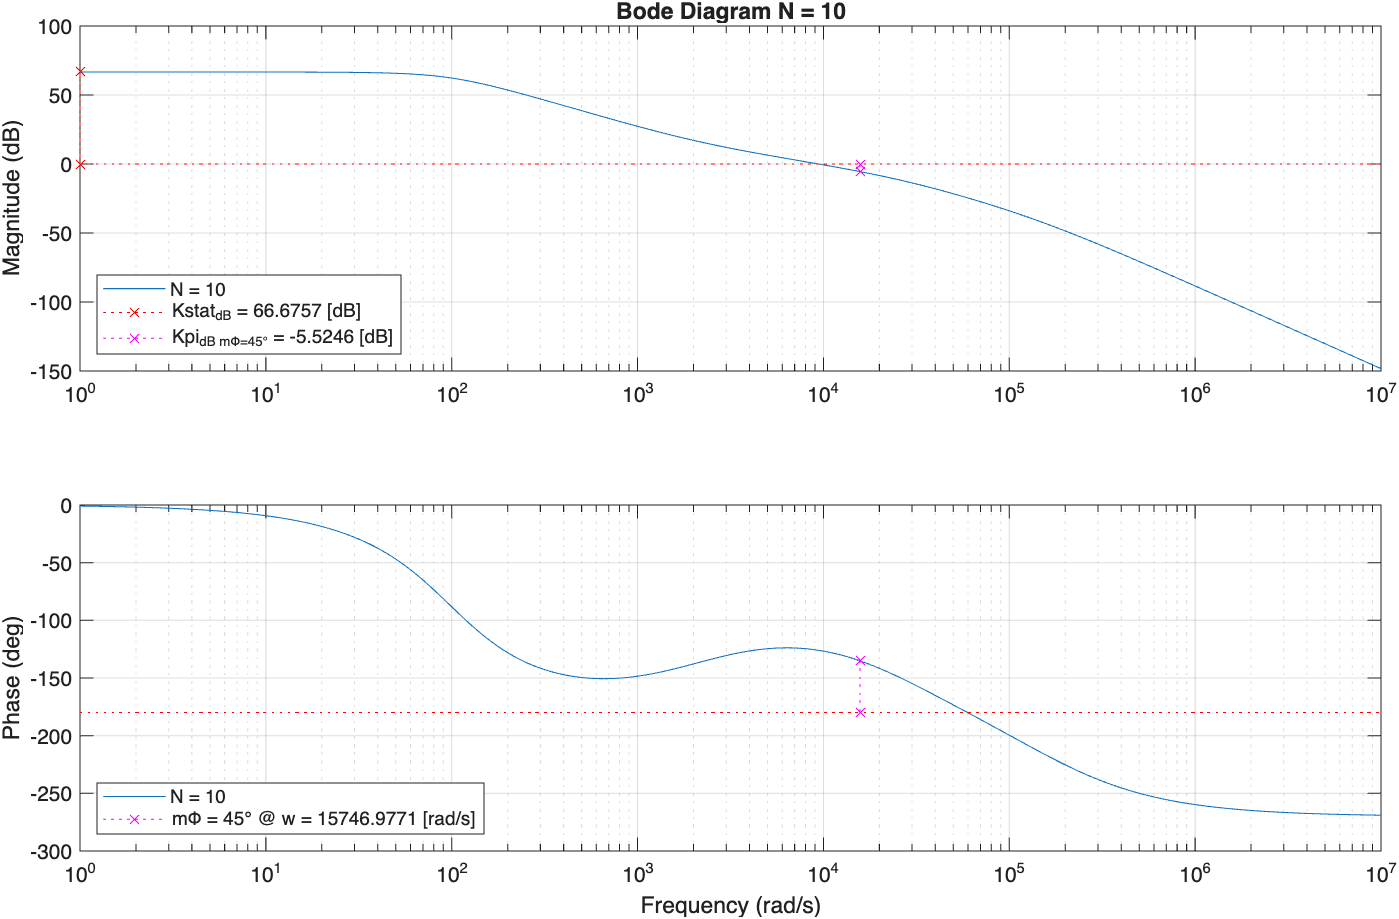
\includegraphics[width=1\linewidth]{assets/Chap4/BodeKpiFaux.png}
    \caption{Identification du gain $K_{pi}$ sans la constante multiplicative}
    \label{fig:BodeKpiFaux}
\end{figure}

\begin{figure}[H]
    \centering
    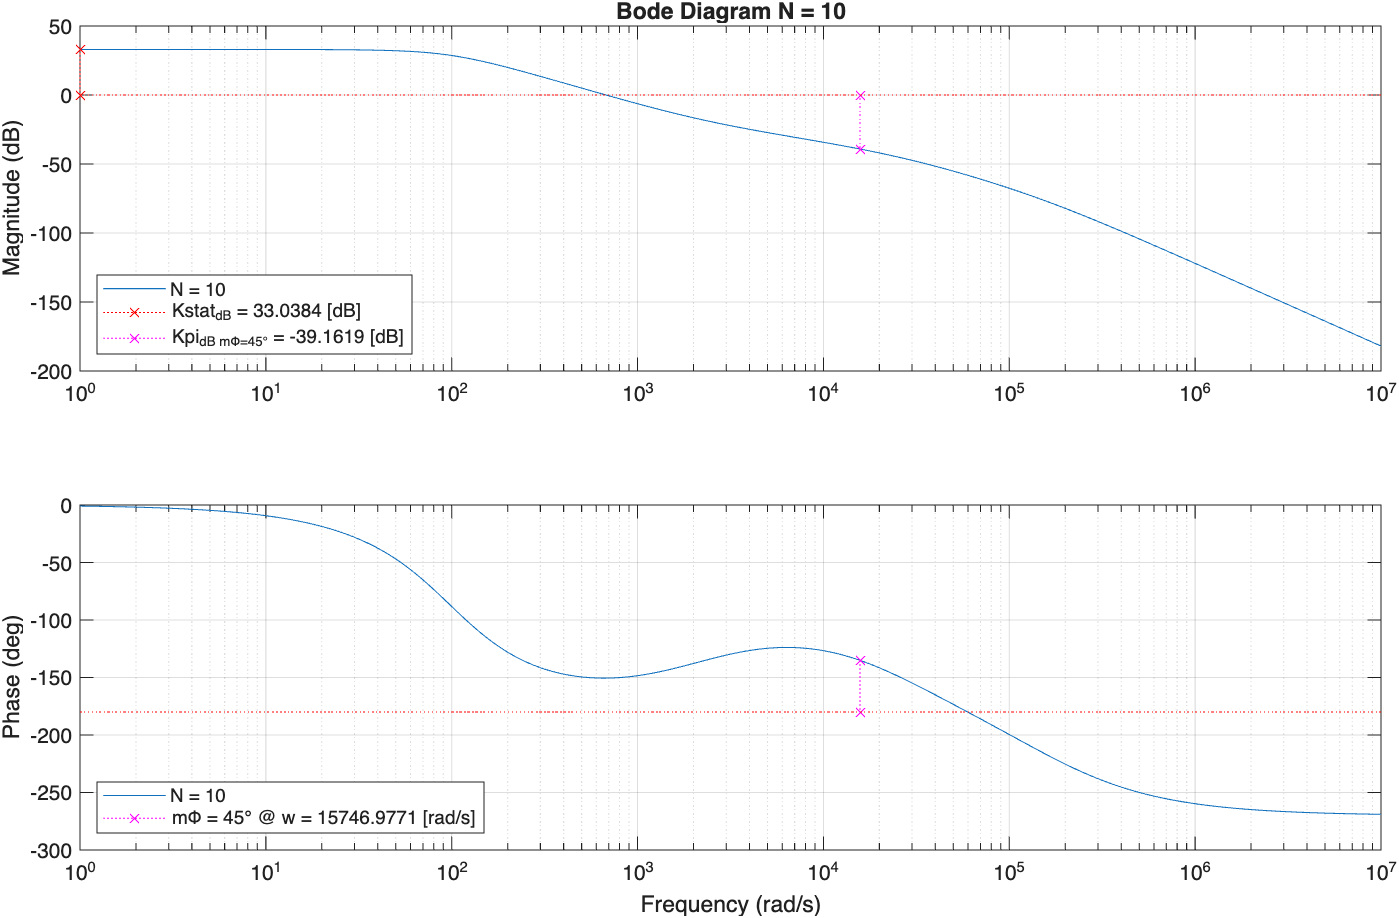
\includegraphics[width=1\linewidth]{assets/Chap4/BodeKpiVrai.png}
    \caption{Identification du gain $K_{pi}$ avec la constante multiplicative}
    \label{fig:BodeKpiVrai}
\end{figure}

Lors de l'implémentation expérimentale, l'introduction de la valeur théorique de 90,96 engendre un plaquage franc de la maquette contre le rail de guidage. Ce phénomène s'explique par le fait que l'étage de puissance a été initialement dimensionné pour le gain inférieur (de l'ordre de 1,89). Avec un gain de 90, une faible erreur statique génère immédiatement une commande en tension saturée. Bien que les limites matérielles du système saturent physiquement la commande à 48~V et 3,5~A, la dynamique excessive requise par ce gain élevé déstabilise le comportement. Les essais physiques mettent en évidence un fonctionnement plus stable pour un gain $K_{pi}$ proche de 1,88.

Il est donc nécessaire d'ajuster expérimentalement ce paramètre dans le code source afin de trouver un compromis offrant une dynamique rapide sans saturer l'actionneur.

\red{Dire que j'ai choisi N = 7 et Kpi a 2 et donner les résultat de tau\_ibf. J'ai choisi cette valeur en essayant plusieurs valeurs. Dire que forcément le choix donnera un tau\_ibf beaucoup plus}

\red{Travail à réaliser par la suite :}
\begin{itemize}
    \item Déterminer expérimentalement la valeur optimale du gain $K_{pi}$.
\end{itemize}

\section{La régulation de position}
La régulation de position est réalisée au moyen d'un retour d'état. Le schéma bloc de cette régulation est défini dans les travaux de Zayadine \cite{Zayadine}, tel que présenté sur la figure \ref{fig:RegPosBloc} :

\begin{figure}[H]
    \centering
    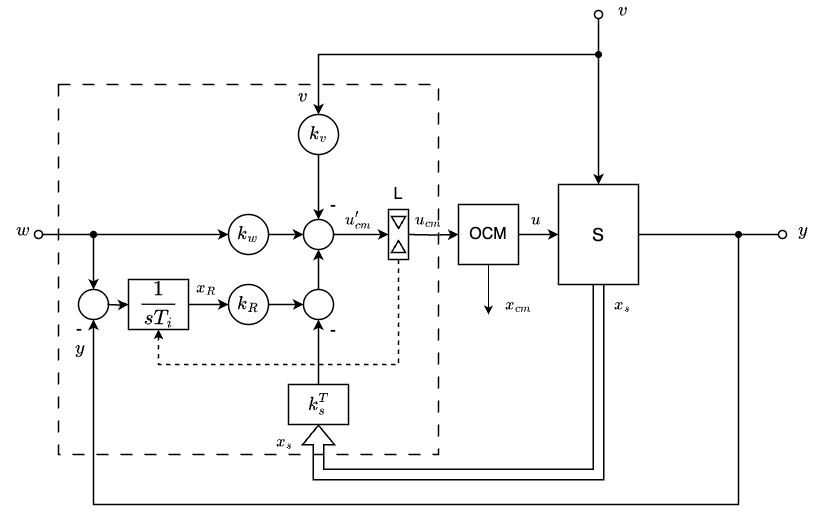
\includegraphics[width=1\linewidth]{assets/Chap4/SchemaMethBuler.png}
    \caption{Schéma bloc de la régulation de position par méthode d'état \cite{Zayadine}}
    \label{fig:RegPosBloc}
\end{figure}

Comme l'illustre la figure \ref{fig:RegPosBloc}, quatre paramètres doivent être dimensionnés : le vecteur de gain de retour d'état $k_s^T$, le coefficient $k_w$, le coefficient $k_R$ et le coefficient $k_v$.

Une simplification est effectuée en regroupant l'ensemble des retards dans un bloc unique, désigné par $G_{pct}$. Celui-ci représente la somme des petites constantes de temps de la régulation de position. Cela inclut la constante de temps de la commande de position $\tau_{m\delta}$, la constante de temps de la régulation de courant en boucle fermée $\tau_{iBF}$, le filtre de Savitzky-Golay caractérisé par $\tau_{vf2}$ et le filtre coupe-bande $\tau_{F_C}$. Ces différents filtres sont modélisés comme de simples retards synthétisés sous forme de filtres passe-bas du premier ordre.

\begin{figure}[H]
    \centering
    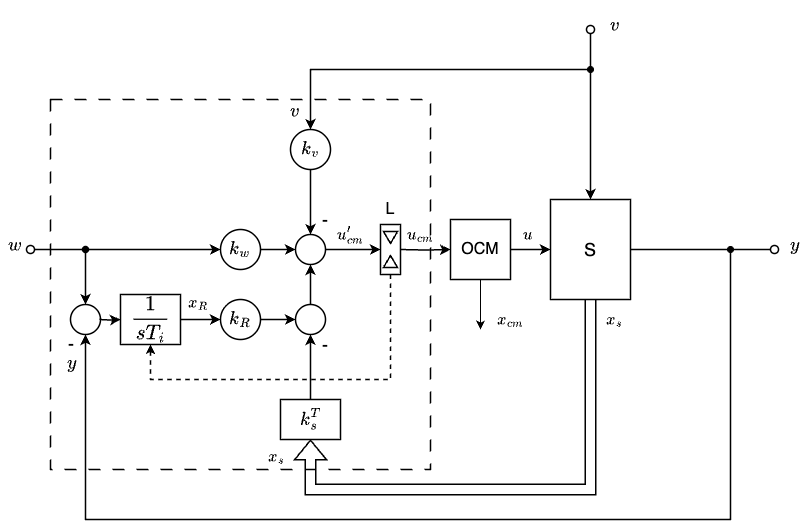
\includegraphics[width=1\linewidth]{assets/Chap4/RegPosBloc.png}
    \caption{Mise en commun des retards}
    \label{fig:MiseCommunRetard}
\end{figure}

Ces constantes de temps sont alors fusionnées en un seul bloc, aboutissant au schéma simplifié de la figure \ref{fig:RegPosBlocSimple} :

\begin{figure}[H]
    \centering
    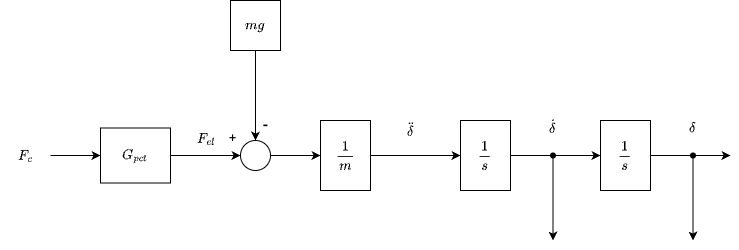
\includegraphics[width=1\linewidth]{assets/Chap4/RegPosBlocSimple.png}
    \caption{Schéma bloc de la régulation de position simplifiée}
    \label{fig:RegPosBlocSimple}
\end{figure}

La fonction de transfert $G_{pct}$ est définie par l'équation \ref{eq:Gpct1} :

\begin{equation}
    G_{pct} = \frac{1}{1 + s \cdot \sum\tau_{pct}} = \frac{1}{1 + s \cdot \left( \tau_{iBF} +\tau_{m\delta} + \tau_{vf2} + \tau_{F_C} \right)}
    \label{eq:Gpct1}
\end{equation}

Les travaux de Yersin \cite{Yersin} permettent d'extraire les valeurs suivantes :

\begin{equation}
    \tau_{m\delta} = 144,7 \text{ $\mu$s}\quad\tau_{vf2} = 65 \text{ $\mu$s}\quad\tau_{F_C} = 3,98 \text{ ms}
\end{equation}

En substituant ces valeurs dans l'équation \ref{eq:Gpct1}, l'expression devient :

\begin{equation}
    G_{pct} = \frac{1}{1 + s \cdot \left( 78,3 + 144,7 + 65 + 3'980 \right)}\cdot 10^{-6} = \frac{1}{1 + s \cdot 4,27\cdot 10^{-3}}
    \label{eq:Gpct1_val}
\end{equation}

L'établissement de la représentation d'état du système peut alors être abordé.

\subsection{Définition de l'espace d'état}
L'analyse des schémas blocs (figures \ref{fig:RegPosBloc} à \ref{fig:RegPosBlocSimple}) met en évidence que la dynamique principale est régie par la loi de Newton, formulée dans l'équation \ref{eq:Newton1}. Pour rappel :

\begin{equation}
    m \cdot \ddot{\delta} =\sum F = F_p - F_{el} = m \cdot g - F_{el}
    \tag{\ref{eq:Newton1}}
\end{equation}

La première étape consiste à définir un vecteur d'état intégrant la position et la vitesse du système, conformément à la figure \ref{fig:RegPosBlocSimple} :

\begin{equation}
    x_s =\left[\begin{matrix} \delta \\ \dot{\delta} \end{matrix}\right]
\end{equation}

Le modèle d'état s'exprime sous la forme générique :

\begin{equation}
    \dot{x}_s = A_s\cdot x_s + B_s\cdot F_{el} + B_{sv}\cdot g
\end{equation}

L'identification des matrices $A_s$, $B_s$ et $B_{sv}$ repose sur la décomposition suivante :

\begin{equation}
    \left\{ \begin{aligned}
         & \dot{\delta} = 0\cdot \delta + 1\cdot \dot{\delta} + 0\cdot F_{el} + 0\cdot g
        \\
         & \ddot{\delta} = 0\cdot \delta + 0\cdot \dot{\delta} - \frac{1}{m}\cdot F_{el} + 1\cdot g
    \end{aligned} \right.
\end{equation}

Les matrices d'état correspondantes sont :

\begin{equation}
    A_s = \begin{bmatrix} 0 & 1 \\ 0 & 0 \end{bmatrix} \quad B_s = \begin{bmatrix} 0 \\ -\frac{1}{m} \end{bmatrix}\quad B_{sv} = \begin{bmatrix} 0 \\ 1 \end{bmatrix}
\end{equation}

L'équation d'observation de la sortie est définie par l'équation \ref{eq:Sortie1} :

\begin{equation}
    y = C_s \cdot x_s + D_s \cdot F_{el} + D_{sv} \cdot g
    \label{eq:Sortie1}
\end{equation}

La sortie du système étant exclusivement la position (voir figure \ref{fig:RegPosBlocSimple}), les matrices d'observation s'écrivent :

\begin{equation}
    C_s = \begin{bmatrix} 1 & 0 \end{bmatrix} \quad D_s =  0 \quad D_{sv} =  0
\end{equation}

Le vecteur des gains de retour d'état s'exprime par :

\begin{equation}
    K_s = \begin{bmatrix} k_\delta \\ k_{\dot{\delta}} \end{bmatrix}
\end{equation}

La modélisation est ensuite étendue au vecteur d'état global du système augmenté :

\begin{equation}
    x = \begin{bmatrix} x_{em} \\ x_s \\ x_r \end{bmatrix} = \begin{bmatrix} x_{em} \\ \delta \\ \dot{\delta} \\ x_r \end{bmatrix}
\end{equation}

La dynamique de ce vecteur global est décrite par la relation :

\begin{equation}
    \dot{x} = A \cdot x + B \cdot F_c + B_w \cdot \delta_c + B_v \cdot g
\end{equation}

Il est nécessaire d'établir les expressions des dérivées de $x_{em}$, $\delta$, $\dot{\delta}$ et $x_r$ en se basant sur le schéma de la figure \ref{fig:RegPosBloc}.\\

La variable $x_{em}$ se déduit de la fonction de transfert $G_{m\delta}$ :

$$G_{m\delta} = \frac{x_{em}}{F_c} = \frac{1}{1 + s \cdot \sum\tau_{pct}}$$

$$\Rightarrow x_{em}(1 + s \cdot \sum\tau_{pct}) = F_c \Rightarrow x_{em} + \dot{x}_{em} \cdot \sum\tau_{pct} = F_c$$

\begin{equation}
    \dot{x}_{em} = \frac{1}{\sum\tau_{pct}} \cdot F_c - \frac{1}{\sum\tau_{pct}} \cdot x_{em}
\end{equation}

L'état $x_{em}$ correspondant physiquement à $F_{el}$, l'équation de l'accélération s'écrit :

\begin{equation}
    \ddot{\delta} = g - F_{el} \cdot \frac{1}{m} = g - x_{em} \cdot \frac{1}{m}
\end{equation}

D'après la figure \ref{fig:RegPosBloc}, l'état de l'intégrateur $x_r$ est régi par :

\begin{equation}
    x_r = \frac{1}{s \cdot T_i} \cdot (\delta_c - \delta) \Rightarrow \dot{x}_r = \frac{1}{T_i} \cdot \delta_c - \frac{1}{T_i} \cdot \delta
\end{equation}

Le regroupement de ces équations permet de définir le système d'état complet :

\begin{equation}
    \left\{
    \begin{aligned}
         & \dot{x}_{em} = -\frac{1}{\sum\tau_{pct}} \cdot x_{em} + 0 \cdot \delta + 0 \cdot \dot{\delta} + \frac{1}{\sum\tau_{pct}} \cdot F_c + 0 \cdot \delta_c + 0 \cdot g
        \\
         & \dot{\delta} = 0 \cdot x_{em} + 0 \cdot \delta + 1 \cdot \dot{\delta} + 0 \cdot F_c + 0 \cdot \delta_c + 0 \cdot g
        \\
         & \ddot{\delta} = -\frac{1}{m} \cdot x_{em} + 0 \cdot \delta + 0 \cdot \dot{\delta} + 0 \cdot F_c + 0 \cdot \delta_c + 1 \cdot g
        \\
         & \dot{x}_r = 0 \cdot x_{em} - \frac{1}{T_i} \cdot \delta + 0 \cdot \dot{\delta} + 0 \cdot F_c + \frac{1}{T_i} \cdot \delta_c + 0 \cdot g
    \end{aligned}
    \right.
\end{equation}

Les matrices du modèle d'état global s'écrivent alors :

\begin{equation}
    A = \begin{bmatrix} -\frac{1}{\sum\tau_{pct}} & 0 & 0 & 0 \\ 0 & 0 & 1 & 0 \\ -\frac{1}{m} & 0 & 0 & 0 \\ 0 & -\frac{1}{T_i} & 0 & 0 \end{bmatrix} \quad B = \begin{bmatrix} \frac{1}{\sum\tau_{pct}} \\ 0 \\ 0 \\ 0 \end{bmatrix}\quad B_w = \begin{bmatrix} 0 \\ 0 \\ 0 \\ \frac{1}{T_i} \end{bmatrix}\quad B_v = \begin{bmatrix} 0 \\ 0 \\ 1 \\ 0 \end{bmatrix}
\end{equation}

L'équation d'observation du système s'écrit :

\begin{equation}
    y = C \cdot x + D \cdot F_c + D_w \cdot \delta_c + D_v \cdot g
\end{equation}

La sortie correspondant à la position, les matrices associées sont :

\begin{equation}
    C = \begin{bmatrix} 0 & 1 & 0 & 0 \end{bmatrix}\quad D = 0\quad D_w = 0 \quad D_v = 0
\end{equation}

La loi de commande (force de consigne) est structurée par la relation suivante :

\begin{equation}
    F_c = K_w \cdot \delta_c + K_v \cdot m - K \cdot x
\end{equation}

Avec :
\begin{itemize}
    \item $K_v$ : Gain de compensation de perturbation.
    \item $K_w$ : Gain de conversion de force.
    \item $K$ : Matrice de gain de retour d'état global.
\end{itemize}

Le vecteur de gain global est défini par :

\begin{equation}
    K = \begin{bmatrix} 0 & K_s & -K_r \end{bmatrix} = \begin{bmatrix} 0 & K_\delta & K_{\dot{\delta}} & -K_r \end{bmatrix}
\end{equation}

La dynamique du système bouclé prend la forme :

\begin{equation}
    \dot{x} = (A - B \cdot K) \cdot x + (B_w + B \cdot K_w) \cdot \delta_c + (B_v - B \cdot K_v) \cdot g = A_G \cdot x + B_G \cdot \delta_c + B_{Gv} \cdot g
\end{equation}

Les matrices d'état du système en boucle fermée sont déterminées par :

\begin{equation}
    B \cdot K = \begin{bmatrix} \frac{1}{\sum\tau_{pct}} \\ 0 \\ 0 \\ 0 \end{bmatrix} \begin{bmatrix} 0 & K_\delta & K_{\dot{\delta}} & -K_r \end{bmatrix} = \begin{bmatrix} 0 & \frac{K_\delta}{\sum\tau_{pct}} & \frac{K_{\dot{\delta}}}{\sum\tau_{pct}} & -\frac{K_r}{\sum\tau_{pct}} \\ 0 & 0 & 0 & 0 \\ 0 & 0 & 0 & 0 \\ 0 & 0 & 0 & 0 \end{bmatrix}
\end{equation}

\begin{equation}
    A_G = A - B \cdot K = \begin{bmatrix} -\frac{1}{\sum\tau_{pct}} & -\frac{K_\delta}{\sum\tau_{pct}} & -\frac{K_{\dot{\delta}}}{\sum\tau_{pct}} & \frac{K_r}{\sum\tau_{pct}} \\ 0 & 0 & 1 & 0 \\ -\frac{1}{m} & 0 & 0 & 0 \\ 0 & -\frac{1}{T_i} & 0 & 0 \end{bmatrix}
\end{equation}

\begin{equation}
    B_G = B_w + B \cdot K_w = \begin{bmatrix} 0 \\ 0 \\ 0 \\ \frac{1}{T_i} \end{bmatrix} + \begin{bmatrix} \frac{1}{\sum\tau_{pct}} \\ 0 \\ 0 \\ 0 \end{bmatrix} K_w = \begin{bmatrix} \frac{K_w}{\sum\tau_{pct}} \\ 0 \\ 0 \\ \frac{1}{T_i} \end{bmatrix}
\end{equation}

\begin{equation}
    B_{Gv} = B_v - B \cdot K_v = \begin{bmatrix} 0 \\ 0 \\ 1 \\ 0 \end{bmatrix} - \begin{bmatrix} \frac{K_v}{\sum\tau_{pct}} \\ 0 \\ 0 \\ 0 \end{bmatrix} = \begin{bmatrix} -\frac{K_v}{\sum\tau_{pct}} \\ 0 \\ 1 \\ 0 \end{bmatrix}
\end{equation}

La sortie du système en boucle fermée est donnée par :
\begin{equation}
    y = C \cdot x + D_G \cdot \delta_c + D_{Gv} \cdot g
\end{equation}

Celle-ci se limitant à la mesure de position, les matrices directes sont nulles :

\begin{equation}
    C = \begin{bmatrix} 0 & 1 & 0 & 0 \end{bmatrix} \quad D_G = 0 \quad D_{Gv} = 0
\end{equation}

\subsection{Placement de pôles}
Afin de concevoir le régulateur, le placement de pôles nécessite la résolution de l'équation caractéristique de la matrice d'état en boucle fermée :

\begin{equation}
    P(s) = \det(s \cdot I - A_G) = 0
\end{equation}

La matrice identité proportionnelle $s \cdot I$ est :

\begin{equation}
    s \cdot I = \begin{bmatrix} s & 0 & 0 & 0 \\ 0 & s & 0 & 0 \\ 0 & 0 & s & 0 \\ 0 & 0 & 0 & s \end{bmatrix}
\end{equation}

Le terme principal du déterminant devient :

\begin{equation}
    s \cdot I - A_G = \begin{bmatrix} s + \frac{1}{\sum\tau_{pct}} & \frac{K_\delta}{\sum\tau_{pct}} & \frac{K_{\dot{\delta}}}{\sum\tau_{pct}} & -\frac{K_r}{\sum\tau_{pct}} \\ 0 & s & -1 & 0 \\ \frac{1}{m} & 0 & s & 0 \\ 0 & \frac{1}{T_i} & 0 & s \end{bmatrix}
\end{equation}

Le calcul de ce déterminant conduit au polynôme caractéristique suivant :

$$\Rightarrow P(s) = \frac{1}{m} \cdot \left( \frac{K_{\dot{\delta}}}{\sum\tau_{pct}} \cdot s + \frac{K_v}{\sum\tau_{pct} \cdot T_i} - \frac{K_\delta}{\sum\tau_{pct}} \cdot s^2 \right) + s \cdot \left( s^3 + s^2 \cdot \frac{1}{\sum\tau_{pct}} \right) = 0$$

$$ \Rightarrow P(s) = -\frac{K_{\dot{\delta}}}{m \cdot \sum\tau_{pct}} \cdot s^2 + \frac{K_\delta}{m \cdot \sum\tau_{pct}} \cdot s + \frac{K_v}{m \cdot \sum\tau_{pct} \cdot T_i} + s^4 + s^3 \cdot \frac{1}{\sum\tau_{pct}} = 0$$

\begin{equation}
    P(s) = s^4 + s^3 \cdot \frac{1}{\sum\tau_{pct}} - s^2 \cdot \frac{K_{\dot{\delta}}}{m \cdot \sum\tau_{pct}} + s \cdot \frac{K_\delta}{m \cdot \sum\tau_{pct}} + \frac{K_v}{m \cdot \sum\tau_{pct} \cdot T_i}
\end{equation}

Cette équation caractéristique doit être identifiée au polynôme cible imposé par les pôles désirés $(p_1, p_2, p_3, p_4)$ :

\begin{equation}
    P(s) = (s - p_1)(s - p_2)(s - p_3)(s - p_4) = s^4 + a_3 \cdot s^3 + a_2 \cdot s^2 + a_1 \cdot s + a_0
\end{equation}

L'identification des coefficients fournit le système suivant :

\begin{equation}
    \left\{
    \begin{aligned}
         & a_0 = -\displaystyle\frac{K_r}{m \cdot T_i \cdot \sum\tau_{pct}} = p_1 \cdot p_2 \cdot p_3 \cdot p_4
        \\
         & a_1 = -\displaystyle\frac{K_\delta}{m \cdot \sum\tau_{pct}} = -(p_1 \cdot p_2 \cdot p_3 + p_2 \cdot p_3 \cdot p_4 + p_1 \cdot p_3 \cdot p_4 + p_1 \cdot p_2 \cdot p_4)
        \\
         & a_2 = -\displaystyle\frac{K_{\dot{\delta}}}{m \cdot \sum\tau_{pct}} = (p_1 \cdot p_2 + p_1 \cdot p_3 + p_1 \cdot p_4 + p_2 \cdot p_3 + p_2 \cdot p_4 + p_3 \cdot p_4)
        \\
         & a_3 = \displaystyle\frac{1}{\sum\tau_{pct}} = -(p_1 + p_2 + p_3 + p_4)
    \end{aligned}
    \right.
\end{equation}

Plusieurs critères de stabilité doivent être respectés pour assurer un placement de pôles fonctionnel. Conformément aux méthodologies établies dans les travaux de Laucella \cite{Laucella} et Yersin \cite{Yersin}, la contrainte majeure stipule que le pôle le plus lent doit satisfaire la condition d'amortissement minimal :

\begin{equation}
    p_{min} \leq \frac{1}{n}\left( \frac{1}{\sum\tau_{pct} - tr\left(A_s\right)} \right) = \frac{1}{4}\left( \frac{1}{4,27\cdot 10^{-3} - 0} \right) = 58.55\text{ $[\frac{1}{s}]$}
\end{equation}

Où $n$ représente l'ordre du système (ici 4) et $tr\left(A_s\right)$ correspond à la trace de la matrice $A_s$ (dont la valeur est nulle pour ce système).\\

Pour déterminer le coefficient $K_w$, le développement de la fonction de transfert en boucle fermée $G_{yw}(s)$ est nécessaire. Elle s'obtient à partir des matrices d'état selon l'équation :

\begin{equation}
    G_{yw}(s) = C\cdot\left( s\cdot I - A_G \right)^{-1}\cdot B_{Gw} + D_G + D_{Gv}
\end{equation}

Le développement de ce produit donne la fonction de transfert suivante :

\begin{equation}
    G_{yw}(s) = \frac{\frac{K_r}{T_i} + s \cdot K_w}{m \cdot \tau_{pct} \cdot \left( s^4 + \frac{1}{\tau_{pct}} \cdot s^3 - \frac{K_{\dot{\delta}}}{m \cdot \tau_{pct}} \cdot s^2 - \frac{K_\delta}{m \cdot \tau_{pct}} \cdot s - \frac{K_r}{T_i \cdot m \cdot \tau_{pct}} \right)}
\end{equation}

L'expression du numérateur révèle la présence d'un zéro dans la fonction de transfert :

\begin{equation}
    \frac{K_r}{T_i} + s \cdot K_w = 0 \rightarrow z_1 = - \frac{K_r}{T_i\cdot K_w}
\end{equation}

Afin d'optimiser le régime transitoire, les modélisations antérieures ont imposé une contrainte spécifique de conception : forcer un pôle du système à être strictement réel et l'annuler par le zéro de la fonction de transfert. Cette approche permet de déterminer la valeur de $K_w$ :

\begin{equation}
    K_w = - \frac{K_r}{p_k\cdot T_i}
\end{equation}

L'algorithme sous Matlab est utilisé pour calculer les différents pôles admissibles. L'ajustement empirique de la valeur du pôle réel ($p_k$) reste nécessaire afin d'obtenir un jeu de paramètres garantissant la stabilité du système en lévitation.

\red{Travail à réaliser :}
\begin{itemize}
    \item Identifier un placement de pôles assurant la robustesse et la stabilité de la régulation
    \item Analyser les simulations afin de trouver un pôle optimal
\end{itemize}

\subsection{Synthèse d'une régulation de position par PID}
La synthèse d'une régulation de position par un régulateur PID a été envisagée. L'objectif de cette démarche est d'obtenir un système dont les composants sont connus et dont l'étude s'avère plus simple qu'une approche par retour d'état. Une fois un comportement satisfaisant obtenu, une analyse des pôles sera réalisée afin de pouvoir effectuer un placement de pôles au sein de la régulation d'état.\\

La synthèse s'appuie sur le schéma bloc présenté dans la figure \ref{fig:PIDBloc} :

\begin{figure}[H]
    \centering
    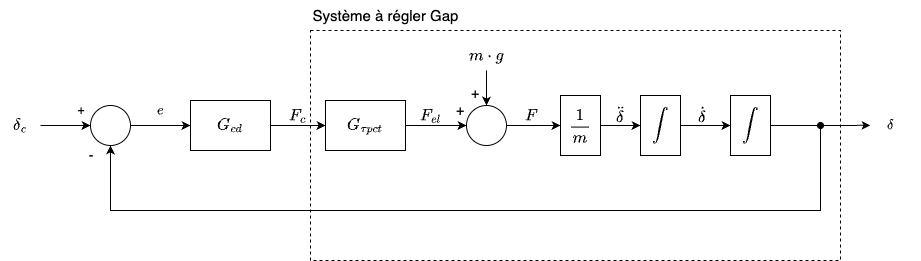
\includegraphics[width=1\linewidth]{assets/Chap4/PIDBloc.png}
    \caption{Schéma bloc de la régulation de position par PID}
    \label{fig:PIDBloc}
\end{figure}

À l'instar de la régulation d'état, l'ensemble des retards a été regroupé au sein d'un bloc unique.

Le système à régler est alors défini par l'équation \ref{eq:Gap} :

\begin{equation}
    G_{ap} = G_{pct}\cdot \frac{1}{m}\cdot s^2 =
    \label{eq:Gap}
\end{equation}

Le diagramme de Bode du système à régler est représenté sur la figure \ref{fig:BodeGap} :

\begin{figure}[H]
    \centering
    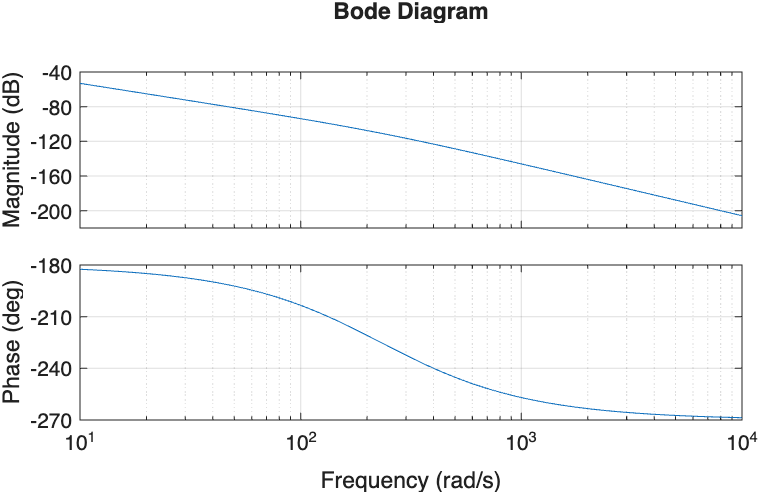
\includegraphics[width=1\linewidth]{assets/Chap4/PID/BodeGap.png}
    \caption{Diagramme de Bode du système à régler $G_{ap}$}
    \label{fig:BodeGap}
\end{figure}

La fonction de transfert du régulateur $G_{cp}$ se définit comme celle d'un PID, exprimée par l'équation \ref{eq:Gcp} :

\begin{equation}
    G_{cp} = K_{pid}\cdot\frac{1 + \tau_i \cdot s + \tau_i \cdot\tau_d\cdot s^2}{\tau_i \cdot s}
    \label{eq:Gcp}
\end{equation}

La synthèse se concentre dès lors sur la détermination des paramètres $K_{pid}$, $\tau_i$ et $\tau_d$.\\

Afin de simplifier cette recherche, le critère de l'optimum symétrique a été employé. La constante de temps de l'action intégrale $\tau_i$ est ainsi fixée à quatre fois la valeur de la constante de temps de l'action dérivée $\tau_d$, comme formulé dans l'équation \ref{eq:OptSym} :

\begin{equation}
    \tau_i = 4\cdot\tau_d
    \label{eq:OptSym}
\end{equation}

Cette méthode permet de réduire l'étude à deux paramètres inconnus : la valeur de $\tau_d$ dans un premier temps, puis le gain $K_{pid}$.\\

La grandeur $\tau_d$ est définie comme le produit de la somme des petites constantes de temps par un coefficient $N$, selon l'équation \ref{eq:TauD} :

\begin{equation}
    \tau_d = N\cdot\sum\tau_{pct} = N\cdot 4.27\cdot 10^{-3}
    \label{eq:TauD}
\end{equation}

À l'image de la synthèse de la régulation de courant, une analyse paramétrique a été menée pour des valeurs de $N$ comprises entre 1 et 20. À l'issue de ces simulations, l'évolution de la bande passante et de l'erreur a été évaluée en fonction de $N$. Seules les configurations garantissant une marge de phase de 45° ont été retenues. Le choix final du paramètre $N$ repose sur un compromis optimal entre la largeur de la bande passante et la prédiction de l'erreur.

Le tracé pour différentes valeurs de $N$ est disponible sur la figure \ref{fig:ChoixNPID} :

\begin{figure}[H]
    \centering
    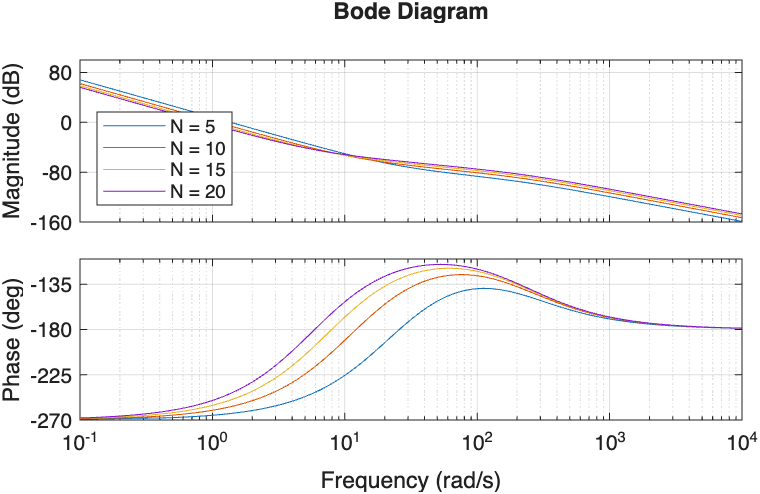
\includegraphics[width=1\linewidth]{assets/Chap4/PID/ChoixN.png}
    \caption{Diagramme de Bode pour différentes valeurs de N}
    \label{fig:ChoixNPID}
\end{figure}

La bande passante est illustrée par la figure \ref{fig:BPPID} :

\begin{figure}[H]
    \centering
    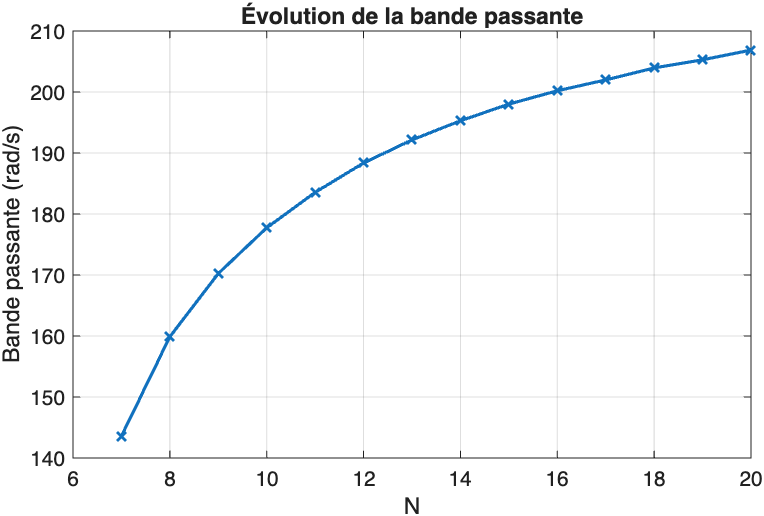
\includegraphics[width=1\linewidth]{assets/Chap4/PID/BP.png}
    \caption{Evolution de la bande-passante en fonction de N}
    \label{fig:BPPID}
\end{figure}

L'erreur est présentée sur la figure \ref{fig:ErrorPID} :

\begin{figure}[H]
    \centering
    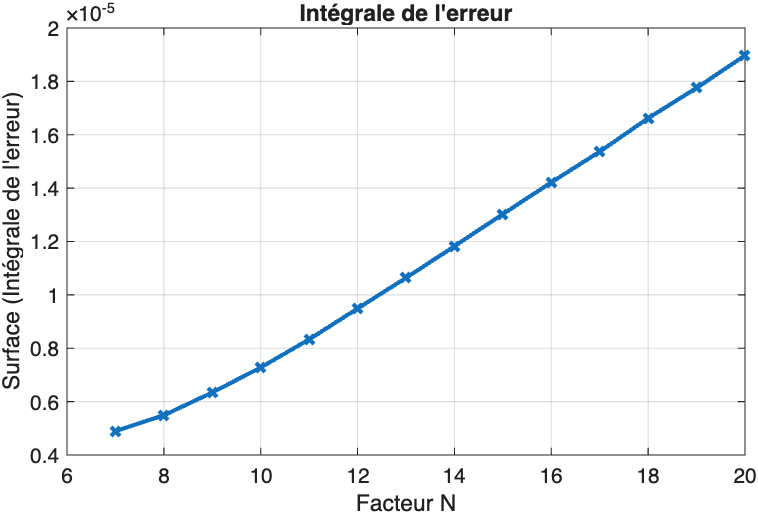
\includegraphics[width=1\linewidth]{assets/Chap4/PID/Erreur.png}
    \caption{Evolution de l'erreur en fonction de N}
    \label{fig:ErrorPID}
\end{figure}

Le choix s'est porté sur la valeur $N=12$, offrant un équilibre satisfaisant entre la bande passante et l'erreur.

Il est alors possible de déterminer le gain $K_{pid}$ en recherchant, pour cette valeur de $N$, la valeur assurant une marge de phase de 45° :

\begin{figure}[H]
    \centering
    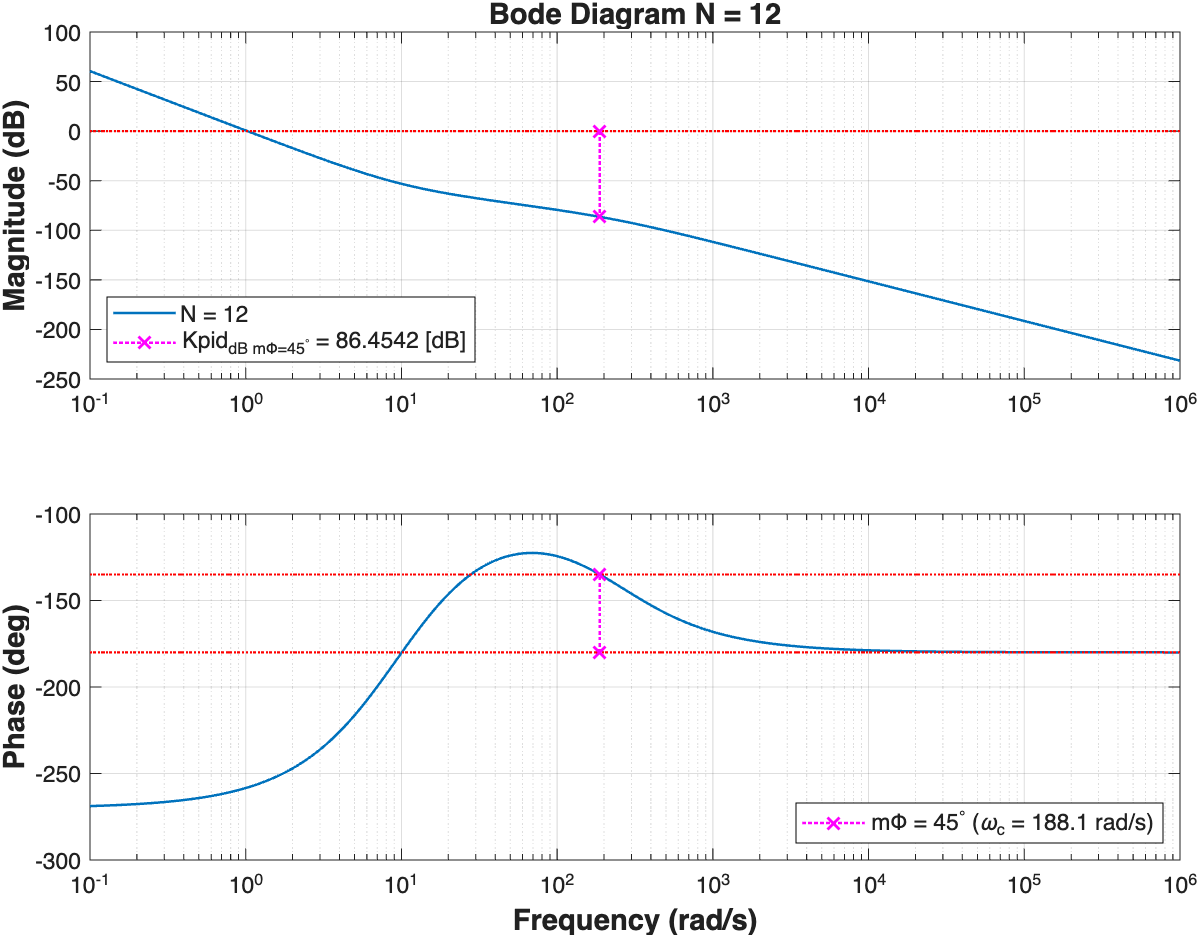
\includegraphics[width=1\linewidth]{assets/Chap4/PID/RechercheKpid.png}
    \caption{Détermination du gain $K_{pid}$}
\end{figure}

Cette configuration détermine les paramètres finaux du régulateur PID, présentés dans l'équation \ref{eq:ParamPID} :

\begin{equation}
    K_{pid} = 20889 \quad \tau_i = 207,7 \text{ ms} \quad \tau_d = 51,9 \text{ ms}
    \label{eq:ParamPID}
\end{equation}

Le diagramme de Bode en boucle ouverte est visible sur la figure \ref{fig:BOPID} :

\begin{figure}[H]
    \centering
    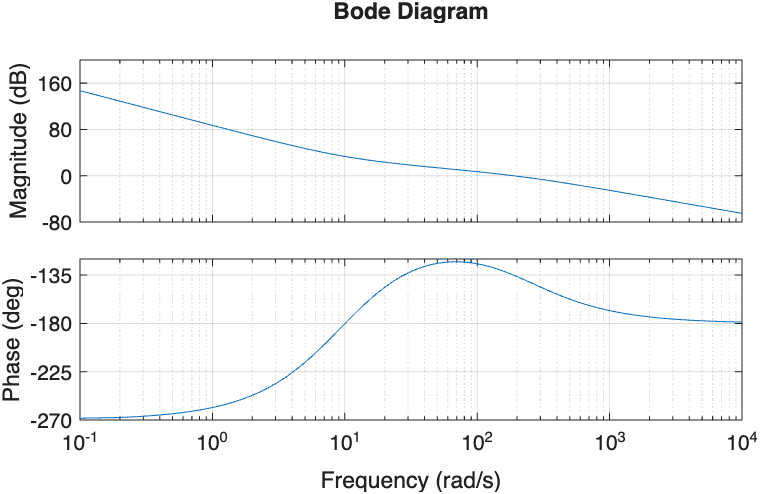
\includegraphics[width=1\linewidth]{assets/Chap4/PID/Gbo.png}
    \caption{Diagramme de Bode de la boucle ouverte}
    \label{fig:BOPID}
\end{figure}

Afin de vérifier le comportement du système, un saut unitaire en boucle fermée a été réalisé. Les résultats sont présentés sur le tracé de la figure \ref{fig:RepIndPID} :

\begin{figure}[H]
    \centering
    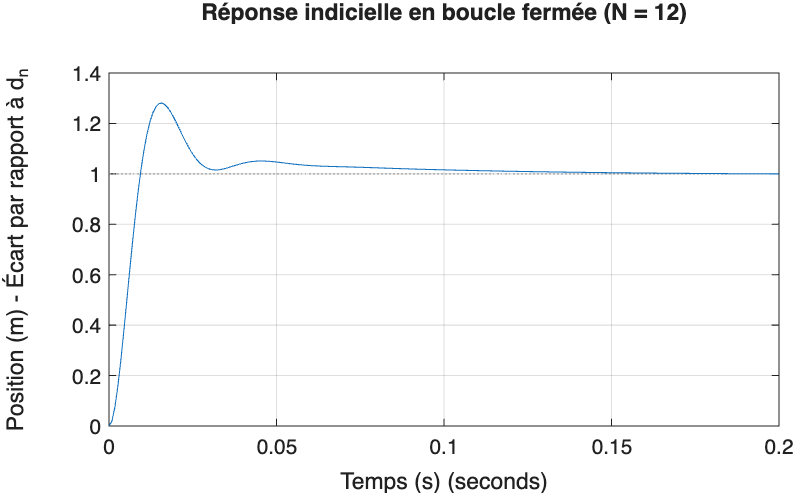
\includegraphics[width=1\linewidth]{assets/Chap4/PID/RepIndi.png}
    \caption{Réponse impulsionnelle du système en boucle fermée}
    \label{fig:RepIndPID}
\end{figure}

Cette réponse indicielle confirme la réactivité adéquate du système vis-à-vis de la maquette.

Cette étude nécessite toutefois d'être validée par des essais physiques sur le démonstrateur, la régulation n'étant pour l'instant qu'au stade de la modélisation.

\begin{itemize}
    \item Réaliser une simulation.
    \item Vérifier la synthèse.
    \item Appliquer les paramètres sur un inducteur pour identifier le comportement réel.
    \item Étendre l'application aux quatre inducteurs.
    \item Déterminer les pôles en boucle fermée.
    \item Transposer les pôles identifiés sur la régulation d'état.
\end{itemize}